\documentclass[a4paper, 10pt]{article}
\usepackage[utf8]{inputenc}
\usepackage{verbatim}
\usepackage{listings}
\usepackage{graphicx}
\usepackage{a4wide}
\usepackage{color}
\usepackage{amsmath}
\usepackage{amssymb}
\usepackage[dvips]{epsfig}
\usepackage[toc,page]{appendix}
\usepackage[T1]{fontenc}
\usepackage{cite} % [2,3,4] --> [2--4]
\usepackage{shadow}
\usepackage{hyperref}
\usepackage{titling}
\usepackage{marvosym }
\usepackage{physics}

\usepackage{subcaption}
\usepackage[noabbrev]{cleveref}
\usepackage{wasysym}
\usepackage{changepage}


\renewcommand{\topfraction}{.85}
\renewcommand{\bottomfraction}{.7}
\renewcommand{\textfraction}{.15}
\renewcommand{\floatpagefraction}{.66}
\renewcommand{\dbltopfraction}{.66}
\renewcommand{\dblfloatpagefraction}{.66}
\setcounter{topnumber}{9}
\setcounter{bottomnumber}{9}
\setcounter{totalnumber}{20}
\setcounter{dbltopnumber}{9}


\setlength{\droptitle}{-10em}   % This is your set screw

\setcounter{tocdepth}{2}

\lstset{language=c++}
\lstset{alsolanguage=[90]Fortran}
\lstset{basicstyle=\small}
\lstset{backgroundcolor=\color{white}}
\lstset{frame=single}
\lstset{stringstyle=\ttfamily}
\lstset{keywordstyle=\color{red}\bfseries}
\lstset{commentstyle=\itshape\color{blue}}
\lstset{showspaces=false}
\lstset{showstringspaces=false}
\lstset{showtabs=false}
\lstset{breaklines}
\title{FYS4411 - Project 1\\
	Variational Monte Carlo}
\author{Daniel Heinesen, Gunnar Lange \& Aram Salihi}
\begin{document}
	\maketitle
	\begin{abstract}
	We present an investigation into bosons trapped in a harmonic oscillator trap. 
	\end{abstract}
	\tableofcontents
	\section{Introduction}
	Confined quantum mechanical systems have received considerable attention in the literature, as they have many possible novel applications, ranging from qubits to energy storage. The existence of Bose-Einstein condensation in gases of certain alkali atoms, has sparked the interest in confined bosonic systems in particular (see e.g. \cite{Nilsen2005}). \\
	\linebreak
	We present an investigation into a system of bosons trapped in a harmonic oscillator well, based on the work by \cite{DuBois2001}. We model our bosons as spheres with radius $a$, and investigate systems both with and without a repulsive interaction preventing them from moving through one another. We then use a variational Monte Carlo simulation to estimate the ground-state energy of our system.\\
	\linebreak
	 We seek to understand how the ground-state energy of the system depends on various parameters such as the number of particles in the system, the shape of the trap and the way we sample in our variational Monte Carlo method. We also investigate metods for quickly determining an approximation to the optimal variational parameter. Finally, we present a brief discussion of onebody densities in our system.
	\section{Theoretical model}
	We investigate bosons in a potential trap. The Hamiltonian of such a system for $N$ bosons is in general given by:
	\begin{equation} \label{eq:general_Hamiltonian}
	H=\sum_{i=1}^N\left(-\frac{\hbar^2}{2m}\nabla_i^2 +V_{ext}(\boldsymbol{r}_i)\right)+\sum_{i<j}^N V_{int}(\boldsymbol{r}_i, \boldsymbol{r}_j)
	\end{equation}
	Where $V_{ext}$ is the external potential, i.e. the potential of the trap, whereas $V_{int}$ is the interal potential, i.e. the interaction potential between the bosons. We wish to approximate the ground state energy of our system described by the Hamiltonian given in equation \ref{eq:general_Hamiltonian}.
	\subsection{The potentials employed}
	\subsubsection{The external potential}
	We will focus on two different trap shapes: spherical and elliptical. The spherical trap can be described by a standard harmonic oscillator potential, which is given by:
	\begin{equation}
	V_{ext}(\boldsymbol{r})=\frac{1}{2}m\omega_{ho}^2 r^2 \quad \mathrm{(spherical\  trap)}
	\end{equation}
	Where $m$ is the mass of the bosons and $\omega$ is a parameter characterizing the strength of the potential (the characteristic frequency of the trap). The elliptical trap, however, is given by:
	\begin{equation}
	V_{ext}(\boldsymbol{r})=\frac{1}{2}m[\omega_{ho}^2 (x^2+y^2)+\omega_z z^2] \quad \mathrm{(elliptical\  trap)}
	\end{equation}
	I.e. we allow the strength of the potential to vary in one direction, which we designate as the $z$-axis.
	\subsubsection{The internal potential}
	We will begin by investigating models where there is no repulsion between the bosons, however, we will later act a repulsive potential that prevents bosons from occupying the same point in space. Here $a$ is a typical diameter of our bosons (the hard-core diameter), which equals the scattering length of the single boson potential. We then define our internal potential as:
	\begin{equation}
	V_{int}(a,|\boldsymbol{r}_i-\boldsymbol{r}_j|)= 
	\begin{cases}
	\infty & \quad |\boldsymbol{r}_i-\boldsymbol{r}_j| \leq  a\\
	0 & \quad |\boldsymbol{r}_i-\boldsymbol{r}_j|>  a\\
	\end{cases}
	\end{equation}
	This potential thus represents the impossibility of bosons to occupy the same point in space.
	\subsection{The variational method}
	\subsubsection{The variational principle}
	To find the ground state energy, $E_0$ of bosons trapped in a potential, we employ the variational method. The variational principle states that:
	\begin{equation}\label{eq:Variational_principle}
	E_0\leq  \frac{\langle \Psi_T |H|\Psi_T \rangle}{\langle \Psi|\Psi\rangle}
	\end{equation}
	Where $H$ is the Hamiltonian of our system and $\Psi_T$ is any trial wavefunction. We therefore choose a functional form for $\Psi_T$, with a number of free parameters. By varying these parameteres, we can find an upper bound for the ground state energy. If our chosen functional form is reasonably close to the exact wavefunction, $\Psi$ of the system, then our estimate for $E_0$ should be reasonably close to the actual ground state energy of our system.
	\subsubsection{Choosing a trial wavefunction}
	As noted above, we must choose our trial wavefunction to be reasonably close to the expected form of the actual position wavefunctions of our system. We note first that the external potential represents a harmonic oscillator. For the harmonic oscillator, it is well known from introductory quantum mechanics that the eigenfunctions are exponential functions for each particle seperately. Note that the elliptic oscillator has a preferred direction (the $z$-axis). We accomodate for this by introducing a parameter $\beta$, representing the asymmetry of the elliptical oscillator. We therefore choose our trial wavefunction for this part of the potential to be:
	\begin{equation}
	h(\boldsymbol{r}_1, ..., \boldsymbol{r}_N, \alpha, \beta)=\prod_{i=1}^N g(\alpha,\beta, \boldsymbol{r}_i)=\prod_{i=1}^N \exp[-\alpha(x_i^2+y_i^2+\beta z_i^2)]=\exp[-\alpha \sum_{i=1}^N (x_i^2+y_i^2+\beta z_i^2)]
	\end{equation}
	Where we now have two variational parameters, $\alpha$ and $\beta$. Here $\beta$ tunes the strength of the potential as a whole, whereas $\beta$ tunes the asymmetry of the spherical oscillator.\\
	\linebreak
	For the internal potential, we expect a function that attenuates our wavefunction down to zero if the distance between any pair of particles becomes less than $a$. We choose this function to be continuous, on physical grounds. A simple choice for such a function is:
	\begin{equation}
	f(a,|\boldsymbol{r}_i-\boldsymbol{r}_j|)= 
	\begin{cases}
	0 & \quad |\boldsymbol{r}_i-\boldsymbol{r}_j| \leq  a\\
	1-\frac{a}{|\boldsymbol{r}_i-\boldsymbol{r}_j|} & \quad |\boldsymbol{r}_i-\boldsymbol{r}_j|>  a\\
	\end{cases}
	\end{equation}
	Putting this together, gives our trial wavefunction as:
	\begin{equation}\label{eq:trial_wavefunction}
	\Psi_T(\boldsymbol{r}_1, \boldsymbol{r}_2, ..., \boldsymbol{r}_N, \alpha, \beta)=\prod_ig(\alpha,\beta, \boldsymbol{r}_i)\prod_{i<j}f(a, |\boldsymbol{r}_i-\boldsymbol{r}_j|)
	\end{equation}
	This is thus the wavefunction that we will be using in equation \ref{eq:Variational_principle} to find our upper bound on the ground state energy.
	\subsection{Analytic results in the simplest case}
	For $\beta=1$ (spherical trap) and $a=0$ (no interaction amongst the particles), our system reduces to a simple harmonic oscillator, for which analytic results are available. For a single particle, the ground-state energy is (according to \cite{Griffiths2004}) given by:
	\begin{equation}
	E=\frac{\hbar \omega d}{2}
	\end{equation}
	Where $d$ is the number of dimensions. For $N$ non-interacting particles this turns into:
	\begin{equation}\label{eq:Exact_Energy_N_particles}
	E=\frac{N\hbar \omega d}{2}
	\end{equation}
	The exact ground-state wavefunction for the harmonic oscillator is (in dimensionless-form) given by:
	\begin{equation}
	\exp\left(-\frac{\sum_{i=1}^d x_i^2}{2}\right)
	\end{equation}
	For $N$ non-interacting particles this turns into:
	\begin{equation}
	\prod_{i=1}^N 	\exp\left(-\frac{\sum_{i=1}^d x_i^2}{2}\right)
	\end{equation}
	Comparing this with our trial wavefunction in equation \ref{eq:trial_wavefunction}, shows that we should expect the ground-state energy to be achieved for:
	\begin{equation}\label{eq:exact_alpha}
	\alpha=0.5
	\end{equation}
	\subsection{Variational Monte Carlo methods}
	Note that equation \ref{eq:Variational_principle} involves two integrals over $3N$ dimensions. This is usually not possible to evaluate analytically for large $N$, and traditional numerical methods such as gaussian quadrature are far too slow in high dimensions to be feasible. We therefore employ variational Monte Carlo methods to help in evaluting these integrals. To do this, we consider these integrals to represents stochastic quantities, and define the probability distribution as:
	\begin{equation}
	P(\boldsymbol{r}_1, \boldsymbol{r}_2,...,\boldsymbol{r}_N, \alpha,\beta)=\frac{|\Psi_T|^2}{\int d\boldsymbol{r}_1d\boldsymbol{r}_2...d\boldsymbol{r_n}|\Psi_T|^2}
	\end{equation}
	Now define a new quantity, the local energy, as:
	\begin{equation}\label{eq:Local_energy_general_expression}
	E_L(\boldsymbol{r}_1, \boldsymbol{r}_2,...,\boldsymbol{r}_N, \alpha,\beta)=\frac{1}{\Psi_T}H\Psi_T
	\end{equation}
	The	expectation value of the Hamiltonian (i.e. the estimate of the energy) now turns into:
	\begin{equation}\label{eq:Expectation_Hamiltonian}
	E[H(\alpha, \beta)]=\int P(\boldsymbol{r}_1, \boldsymbol{r}_2,...,\boldsymbol{r}_N, \alpha,\beta)E_L(\boldsymbol{r}_1, \boldsymbol{r}_2,...,\boldsymbol{r}_N, \alpha,\beta)d\boldsymbol{r}_1d\boldsymbol{r}_2...d\boldsymbol{r}_N\approx \frac{1}{M}\sum_{i=1}^M E_{L,i}
	\end{equation}
	Where now $M$ is the number of Monte Carlo cycles, whereas $E_{L,i}$ is the local energy computed in the i-th Monte Carlo step. Note that the quality of this approximation is contingent upon our ability to sample our space. We employ two different algorithms for sampling our coordinate space.
	\subsubsection{The Metropolis algorithm}
	To move from one Monte Carlo step to the other, we will employ the Metropolis algorithm, as described in \cite{Hjorth-Jensen2015}. The alogrithm works by sampling the probability distribution, but adding a bias to sample mostly in the regions where the probaility distribution actually is large, to avoid wasting CPU cycles. The algorithm works by proposing a step:
	\begin{equation}
	\boldsymbol{r}_{p, new}=\boldsymbol{r}_p+r \cdot \boldsymbol{dx}
	\end{equation}
	Where $r$ is a random number in $[0,1]$ and $\boldsymbol{dx}$ is a chosen step vector. We then compute the ratio:
	\begin{equation}
	w=\frac{P(\boldsymbol{r}_1, ..., \boldsymbol{r}_{p,new}, ..., \boldsymbol{r}_n)}{P(\boldsymbol{r}_1, ..., \boldsymbol{r}_{p}, ..., \boldsymbol{r}_n)}=\frac{|\Psi_T(\boldsymbol{r}_1, ..., \boldsymbol{r}_{p,new}, ..., \boldsymbol{r}_n)|^2}{|\Psi_T(\boldsymbol{r}_1, ..., \boldsymbol{r}_{p}, ..., \boldsymbol{r}_n)|^2}
	\end{equation}
	This ratio determines whether the new position has a higher or lower value of the PDF than the old position. We then accept the move if and only if $w\geq r$, where $r\in [0,1]$ is a uniformly distributed random variable. This ensures that some steps that decrease the value of the PDF are accepted (giving a spread of value), but that we mostly sample where the PDF is large (which avoids wasting CPU cycles).
	\subsubsection{The Metropolis-Hastings algorithm (importance sampling)}\label{sec:Metropolis_Hasting_Sampling}
	The simple Metropolis algorithm described above assigns no preferred direction $\boldsymbol{dx}$ for the proposed step. This can be improved by adding a force term, "pushing" the Monte Carlo loop towards the region where the PDF is large. This is described in further detail in \cite{Hjorth-Jensen2015}, where it is shown that the expression fur such a quantum force is given, for particle $k$, by:
	\begin{equation}
	\boldsymbol{F}_k(\boldsymbol{r}_1, ..., \boldsymbol{r}_N)=2\frac{1}{\Psi_T}\nabla_k \Psi_T
	\end{equation}
	We compute explicitly the expression for $\boldsymbol{F}$, using the trial wavefunction in equation \ref{eq:trial_wavefunction}, in appendix \ref{ap:analytic_expression_for_the_local_energy_and_quantum_force}. This gives:
	\begin{equation}
	\boldsymbol{F}_k=	 -4\alpha\boldsymbol{Q}_{k} +
	2\sum_{j \neq k}\frac{\boldsymbol{r}_{k} - \boldsymbol{r}_{j}}{r_{kj}}u'(r_{kj})
	\end{equation}
	A more detailed analysis (given in \cite{Hjorth-Jensen2015}) shows that the correct way to incorporate such a term into the Metropolis algorithm is by adding a transition probability term given by the Green's functions:
	\begin{equation}\label{eq:Greens_Function}
	G(\boldsymbol{r}_1,...,\boldsymbol{r}_N,\boldsymbol{r'}_1,...,\boldsymbol{r'}_N)=\frac{1}{(4\pi D \Delta t)^{3/2}}\sum_{i=1}^N \exp \left(-\frac{(\boldsymbol{r}_i-\boldsymbol{r'}_i-D\Delta t\boldsymbol{F}_i(\boldsymbol{r}'_1,...,\boldsymbol{r}'_N))^2}{4D\Delta t}\right)
	\end{equation}
	Where $\boldsymbol{r}_i$ are the coordinates prior to the move and $\boldsymbol{r'}_i$ are the coordinates after the move, $D$ is a diffusion constant (equal to $1/2$) and $\Delta t$ is a step parameter that we tune. The effect of this term is to modulate the acceptance probability, $w$. This term is now given by:
	\begin{equation}
	w(\boldsymbol{r}_1,...,\boldsymbol{r}_N,\boldsymbol{r'}_1,...,\boldsymbol{r'}_N)=\frac{G(\boldsymbol{r}_1,...,\boldsymbol{r}_N,\boldsymbol{r'}_1,...,\boldsymbol{r'}_N)|\Psi_T(\boldsymbol{r}_1,...,\boldsymbol{r}_N)|^2}{G(\boldsymbol{r'}_1,...,\boldsymbol{r'}_N,\boldsymbol{r}_1,...,\boldsymbol{r}_N)|\Psi_T(\boldsymbol{r'}_1,...,\boldsymbol{r'}_N)|^2}
	\end{equation}
	Which leads to the modified Metropolis algorithm, the Metropolis-Hastings algorithm, where a move is accepted if and only if $w\geq r$ where $r\in [0,1]$ again is a uniformly distributed random variable. This method is computationally far more expensive than the brute-force Metropolis algorithm, but it leads to a  significantly larger number of accepted steps.
	\subsection{The local energy}
	Note that in  order to estimate the expectation value of the Hamiltonian we must, according to equation \ref{eq:Expectation_Hamiltonian} compute the local energy, given by equation \ref{eq:Local_energy_general_expression}, in every Monte Carlo step. The local energy can be rewritten as:
	\begin{equation}
	E_L=\frac{1}{\Psi_T}H\Psi_T =\sum_{i=1}^N\left(-\frac{\hbar^2}{2m\Psi_T}\nabla_i^2 \Psi_T+V_{\mathrm{ext}}(\boldsymbol{r}_i)\right)+\sum_{i<j}^N V_{\mathrm{int}}
	\end{equation}
	We compute this numerically, but we also include an analytic computation, using our trial wavefunction $\Psi_T$ defined in equation \ref{eq:trial_wavefunction}. This is done in detail in appendix \ref{ap:analytic_expression_for_the_local_energy_and_quantum_force}, and gives:
	\begin{align}\label{eq:Local_energy_all}
	\begin{split}
	E_{L} = -\frac{\hbar^{2}}{2m}\sum_{k}\left[
	4\alpha^{2}\boldsymbol{Q}_{k}^{2} - 4\alpha\boldsymbol{Q}_{k} + \sum_{j \neq k}\left(\frac{\boldsymbol{r}_{k} - \boldsymbol{r}_{j}}{r_{kj}}u'(r_{kj})\right)\right.
	\\ \left. + \sum_{i,j \neq k}\left(\frac{\boldsymbol{r}\cdot\boldsymbol{r} + \boldsymbol{r}_{j}\cdot\boldsymbol{r}_{i} - \boldsymbol{r}_{j}\cdot\boldsymbol{r}_{k} -\boldsymbol{r}_{k}\cdot\boldsymbol{r}_{i}}{r_{ki}r_{kj}}u'(r_{ki})u'(r_{kj})\right)\right.
	\\
	\left. + \sum_{j \neq k}\left(u''(r_{kj} + \frac{2}{r_{kj}}u'(r_{kj}))\right)\right]
	+ \sum_{k}V_{ext}(\boldsymbol{r}_{k}) + \sum_{i < j}V_{int}(\boldsymbol{r}_{i}, \boldsymbol{r}_{j})
	\end{split}
	\end{align}
	 Where $\boldsymbol{Q}_{k} = \left(x_{k}\hat{i} + y_{k}\hat{j} + \beta z_{k}\hat{k}\right)$.	
	\subsection{Gradient descent method to find the optimal parameter $\boldsymbol{\alpha}$}\label{sec:Gradient_descent_theory}
	To reduce our search space, we use a minimization method to find an approximation to the optimal variational parameter, $\alpha$. This minimization method is run with relatively few Monte Carlo steps, and once an approximate optimal parameter is found, we perform the analysis with many Monte Carlo steps. As our parameter space is one-dimensional ($\alpha$ is the only variational parameter), we choose to implement a simple gradient descent algorithm. This is implemented as follows:
	\begin{equation}
	\alpha_{n+1}=\alpha_n-\gamma_n \frac{\partial E_L}{\partial \alpha} (\alpha_n)
	\end{equation}
	We choose an initial $\alpha_0$ close to the correct $\alpha$ from the non-interacting case, and then iteratively follow wherever the gradient is lower. We use an adaptive step-size, which decreases as the difference between subsequent gradients decrease (i.e. as we get closer to the minimum). We follow \cite{doi:10.1093/imanum/8.1.141} for this, using:
	\begin{equation}
	\gamma_n=\frac{(\alpha_n-\alpha_{n-1})+\epsilon}{[\frac{\partial E_L}{\partial \alpha}(\alpha_n)-\frac{\partial E_L}{\partial \alpha}(\alpha_{n-1})]}
	\end{equation}
	Where we, however, implement add an additional parameter $\epsilon$ (compared to \cite{doi:10.1093/imanum/8.1.141}) to ensure that we do not get stuck at the same $\alpha$ values. Furthermore, we also implement an additional test that checks if $\frac{\partial E_L}{\partial \alpha}(\alpha_n)-\frac{\partial E_L}{\partial \alpha}(\alpha_{n-1})$ is less than a treshold, in which case we reset $\gamma$ to the initial guess $\gamma_0$.\\
	\linebreak	
	To implement this, we require the derivative of the local energy. We show in appendix \ref{ap:derivative_of_local_energy} that this is given by:
	\begin{equation}
	\frac{\partial E_L}{\partial \alpha}(\alpha_n)=2\left(\big\langle \frac{1}{\Psi_T}\frac{\partial \Psi_T}{\partial \alpha}E_L[\alpha_n]\big\rangle-\big\langle \frac{1}{\Psi_T}\frac{\partial \Psi_T}{\partial \alpha}\big\rangle \big\langle E_L[\alpha_n]\big\rangle\right)
	\end{equation}
	Where we note that both the local energy and the wavefunction depend on $\alpha$.
	\subsection{One-body densities}
	We are interested in investigating the probability of finding a single particle at a distance $r$ from the origin of our system. This is an important quantity, as it can be measured experimentally. We approach this through the concept of the one-body density. The one-body density is defined by:
	\begin{equation}\label{eq:OneBodyDensity}
	\rho(\boldsymbol{r_1})=\int d\boldsymbol{r_2}...d\boldsymbol{r_N}|\Psi_T(\boldsymbol{r_1},\boldsymbol{r_2},...,\boldsymbol{r_N})|^2
	\end{equation}
	Where $\boldsymbol{r_1}$ is the position of any particle. The integral is evaluated using Monte Carlo integration, as described in further detail in section \ref{sec:MetOneBody}.
	
	
	
	
	\section{Methods}\label{Method_section}
	\subsection{A note on units}
	The scattering-length for a typical BEC condensate atom is somewhere in the range $85<a<140a_0$, where $a_0$ is the Bohr radius. The characteristic trap length (at 0 K), however, is $a_{ho}=(\hbar/m\omega)^{1/2}\approx 10^{4}$Å$-2\cdot 10^{4}$Å. We introduce length units of $a_{ho}$ and energy units of $\hbar \omega$. We show in appendix \ref{ap:dimensionless_hamiltonian} that, using these units, the Hamiltonian can be rewritten as:
	\begin{equation}\label{eq:Hamiltonian_dimensionless}
	H=\sum_{i=1}^N\left(-\nabla_i^2 + x_i^2+y_i^2+\gamma z_i^2\right)+\sum_{i<j}V_{int}(\boldsymbol{r}_i, \boldsymbol{r}_j)
	\end{equation}
	Where $\gamma=\omega_z/\omega$.
	\subsection{Implementing the interacting case}
	To implement the interacting case ($a\neq 0$), we follow the parameters used by \cite{Nilsen2005}. We therefore let $a=0.0043$ and $\omega_z=\beta=2.82843$. We find the optimal $\alpha$ in the interacting case by using the gradient descent method described in section \ref{sec:Gradient_descent_theory}, using $100$ times fewer Monte Carlo cycles in the gradient descent calculations compared to the full simulation.
	\subsection{Outline of the structure of our program}
	Our program uses the \texttt{Eigen} library in \texttt{C++} to keep track of the matrices. We implement three main classes:\\
	\paragraph{\texttt{main.cpp}}
	This class reads in the parameters from an input file, sets up parallelization in MPI and starts a new simulation.\\
	\linebreak
	\paragraph{\texttt{simulation.cpp}}
	This class contains the gradient descent method, as well as a method that actually runs the main Monte Carlo loop. The onebody densities are also computed in this class.\\
	\linebreak
	\paragraph{system.ccp}
	This class distributes the particles in the system, sets up the grid, calculates the wavefunction, proposes new steps and checks the acceptance of the steps. 
	\subsection{Proposing a new position}
	To propose a new step, we use a different method for the brute force method versus the importance sampling method. For the brute force method, we propose a new step as:
	\begin{equation}
	\boldsymbol{r}^i_{\mathrm{new}}=\boldsymbol{r}^i_{\mathrm{old}}+\boldsymbol{\xi} dx
	\end{equation}
	Where $\boldsymbol{r}^i_{\mathrm{old}}$ is the previous position of particle $i$ and $\boldsymbol{xi}$ is a normally distributed variable with mean $0$ and standard deviation $1$. We tune the parameter $dx$ for the brute force simulation, and find that we get good results for $dx=1.5$.\\
	\linebreak
	For importance sampling, however, we propose a different step to keep the statistics consistent (as discussed in \cite{Jonsson2018}). The new step is then given by:
	\begin{equation}
	\boldsymbol{r}^i_{\mathrm{new}}=\boldsymbol{r}^i_{\mathrm{old}}+\boldsymbol{\xi} \sqrt{dt}+D\boldsymbol{F}_idt
	\end{equation}
	Where $F_i$ is the quantum force on particle $i$ and $D$ is the diffusion parameter, discussed in section \ref{sec:Metropolis_Hasting_Sampling}. The parameter $dt$ is the same parameter used in the Greens function (equation \ref{eq:Greens_Function}), and we find it by looking at the energy for the exactly solvable system for different $dt$.
	\subsection{Finding the optimal step size}\label{sec:finding_optimal_step_size}
	For the brute-force Monte Carlo sampling, we must estimate an optimal step size, $d x$, with which to move our step. For the Monte Carlo simulation with importance sampling, we must similarly estimate the parameter $d t$. These step sizes should ensure that:
	\begin{itemize}
		\item The simulation quickly converges to the correct energy
		\item The variance quickly stabilizes
	\end{itemize}
	To find these properties, we look at how the variance and the mean of the local energy (across every Monte Carlo sample) varies as we increase the number of Monte Carlo cycles. We investigate various values of $dx$ (respectively $dt$). For each of these values, we ensure that we manage to hit an energy minimum at $\alpha=0.5$ in the noninteracting case.\\
	\linebreak
	We measure the variance in the standard way (i.e. not using blocking), as blocking requires the number of steps to be a power of $2$. We do this for the noninteracting system, using $\alpha=0.45$ (as the exact $\alpha$ gives essentially $0$ variance). \\
	\linebreak
	We then choose the $dx$ (respectively $dt$) that ensure that the variance and the mean quickly stabilize.
	\subsection{Statistical treatment of the data}\label{sec:Blocking}
	We wish to estimate the statistical errors of our estimate of the local energy. As subsequent values for the local energy are based on the previous values of the local energy, we are dealing with a correlated time series. The normality assumptions usually employed when generating confidence intervals therefore does not hold. Instead, we use blocking to estimate the error in our energy. A detailed mathematical treatment of this method is found in \cite{Jonsson2018}. We therefore present only the algorithm. Assume that we have $n$ observations $Q^0=\{Q_1^0,...,Q_n^0\}$ of the local energy, and we wish to estimate the variance of the local energy. The uncorrelated estimator for the standard deviation is given by:
	\begin{equation}
	s=\sqrt{\frac{1}{n-1}\sum_{i=1}^n (Q_i-\overline{Q})^2}
	\end{equation}
	Where $\overline{Q}$ is the mean of the local energy estimates. This expression is only valid in the uncorrelated case, however. The idea of blocking is to perform iterative transformations of the data, until the covariance of the data is approximately zero. Specifically, the transformation that we will be implementing is the following:
	\begin{equation}
	Q^i \rightarrow Q^{i+1}: Q^{i+1} = \left\{ \frac{Q^i_1+Q^i_2}{2}, \frac{Q^i_3+Q^i_4}{2},...,\frac{Q^i_{n-1}+Q^i_{n}}{2}\right\}
	\end{equation}
	We choose $n$ to be a power of a, i.e. $n=2^d$. Thus, we can perform this transformation a maximum of $d$ times. We now define an estimator for the covariance bewteen observations that are distance $h$ apart by:
	\begin{equation}
	\hat{\gamma^k}(h)=\frac{1}{n}\sum_{i=1}^{n-h}(Q_i^k-\overline{Q}^k)(Q_{i+h}^k-\overline{Q}^k)
	\end{equation}
	We are interested in knowing when $\gamma^k(1)\approx 0$. This can be found by hand, simply by realizing that the transformation $Q^i \rightarrow Q^{i+1}$ described above preserves the variance of the data. It is shown in \cite{Jonsson2018} that $\gamma^k(1) \rightarrow 0$ for successive iterations, and therefore a plot of the empirical variance as a function of iterations should eventually stabilize, giving the variance. \\
	\linebreak
	We use an alternative, automatic, approach to estimate when the covariance is small. This is based on comparing our results to a $\chi^2$ distribution, and is described further in \cite{Jonsson2018}.
	\subsection{Implementing the onebody density}\label{sec:MetOneBody}
	To compute the one-body density defined by equation \ref{eq:OneBodyDensity}, we must compute the integral. We show that in appendix \ref{ap:approximte_onebody_density} that, if we only consider the radial distribution of the onebody density, this integral can be discretized as:
	\begin{equation}
		\rho(r_i)\approx \frac{N_i}{4\pi r_i^2 \Delta r}
		\end{equation}
		Where $N_i$ is the number of particles in the spherical shell with radius $r_i$ to $r_i+\Delta r$. Thus, to compute the onebody density, we run our Monte Carlo simulation and check in which shell the particle that we move at every step is located. We also check numerically that the normalization is correct.
	
	\section{Results}
	\subsection{Finding the optimal step size}
We plot the mean and the variance for various steps sizes, as discussed in section \ref{sec:finding_optimal_step_size}. This gives the plot shown in figure \ref{fig:find_dx_noimportance} for the brute force sampling.
	\begin{figure}[ht!]
		\centering
			\centering
			\begin{subfigure}{.5\textwidth}
				\centering
				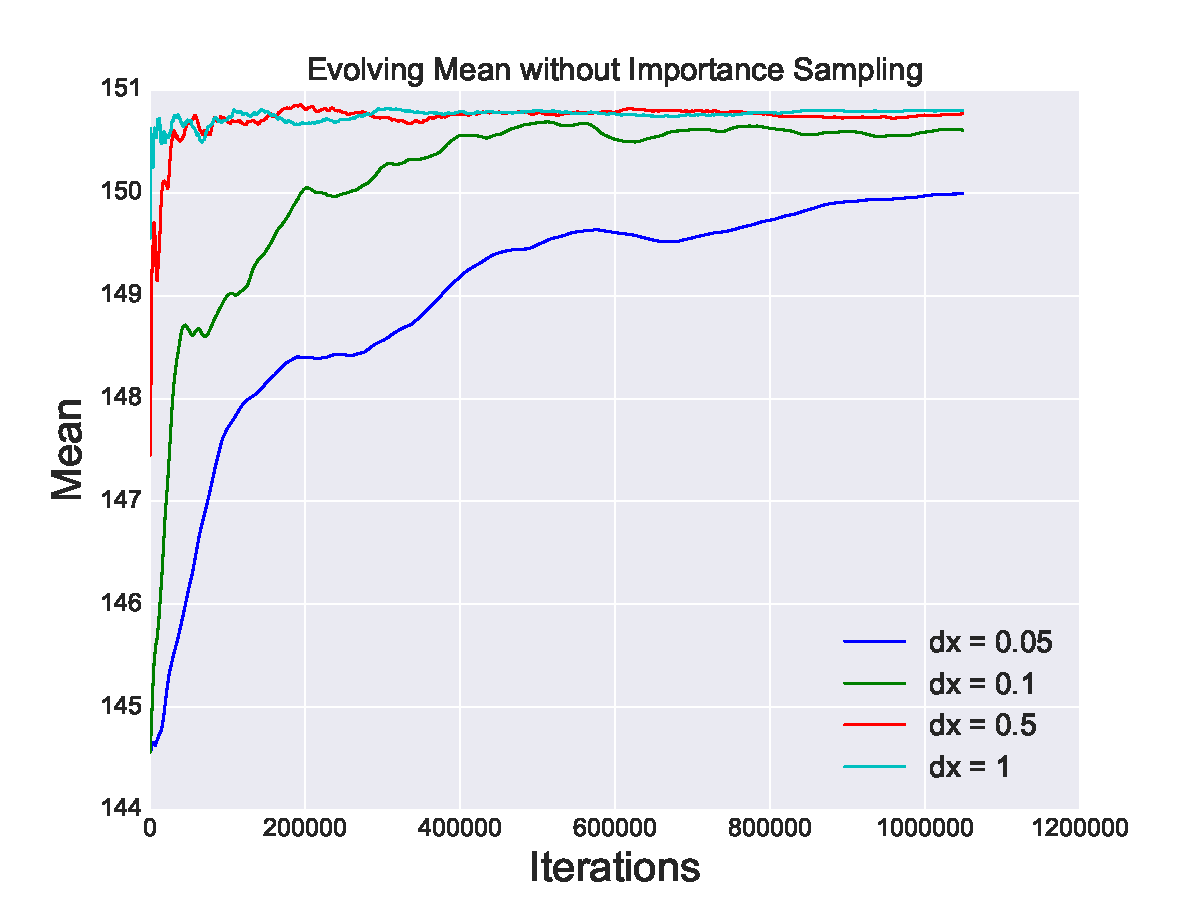
\includegraphics[width=.8\linewidth]{../Results/EvoMean.pdf}
				\caption{Mean energy}
			\end{subfigure}%
			\begin{subfigure}{.5\textwidth}
				\centering
				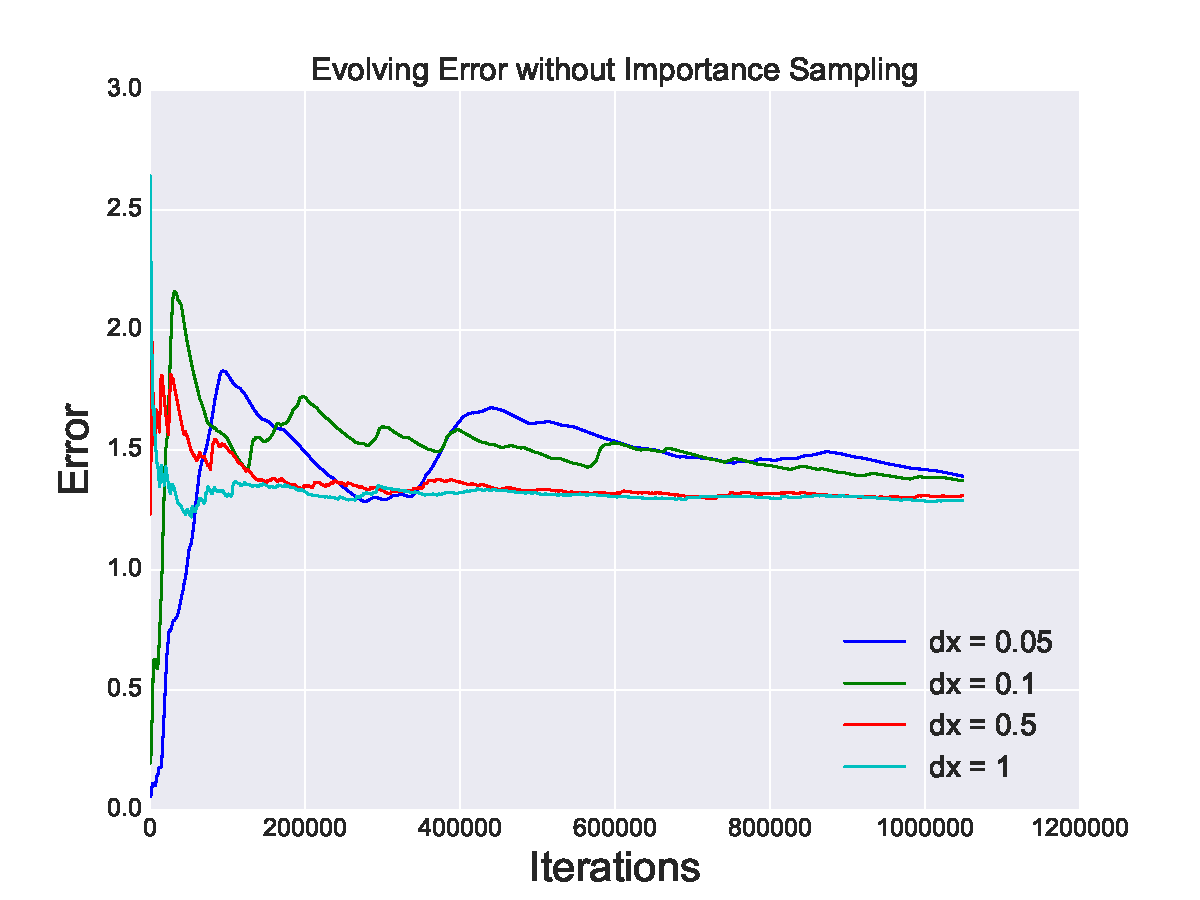
\includegraphics[width=.8\linewidth]{../Results/EvoStd.pdf}
				\caption{Standard deviation of the energy}
			\end{subfigure}
			\caption{Mean energy and standard deviation of the energy as a function of Monte Carlo cycles for various step sizes, $dx$. This was done without importance sampling in three dimensions, using $N=100$, $a=0$ (noninteracting), $\alpha=0.45$, $\omega_z=1$, $\beta=1$,}\label{fig:find_dx_noimportance}
	\end{figure}
	As discussed further in section \textbf{SECTION}, we choose $dx=0.5$ as our parameter for the brute-force case.\\
	\linebreak
	We produce a similar plot for the case with importance sampling. This gives the plots shown in figure \ref{fig:find_dx_importance}.
		\begin{figure}[ht!]
			\centering
			\centering
			\begin{subfigure}{.5\textwidth}
				\centering
				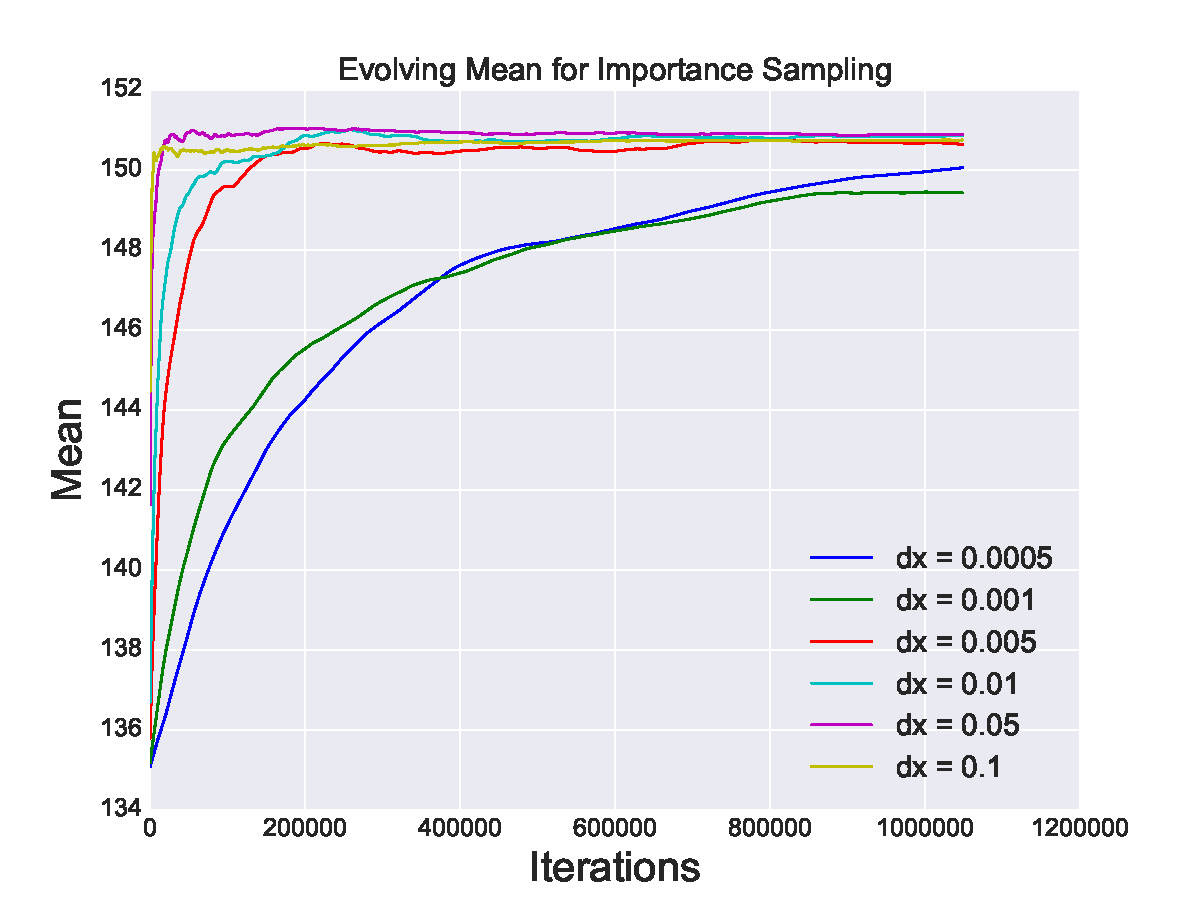
\includegraphics[width=.8\linewidth]{../Results/EvoMeanIS.pdf}
				\caption{Mean energy}
			\end{subfigure}%
			\begin{subfigure}{.5\textwidth}
				\centering
				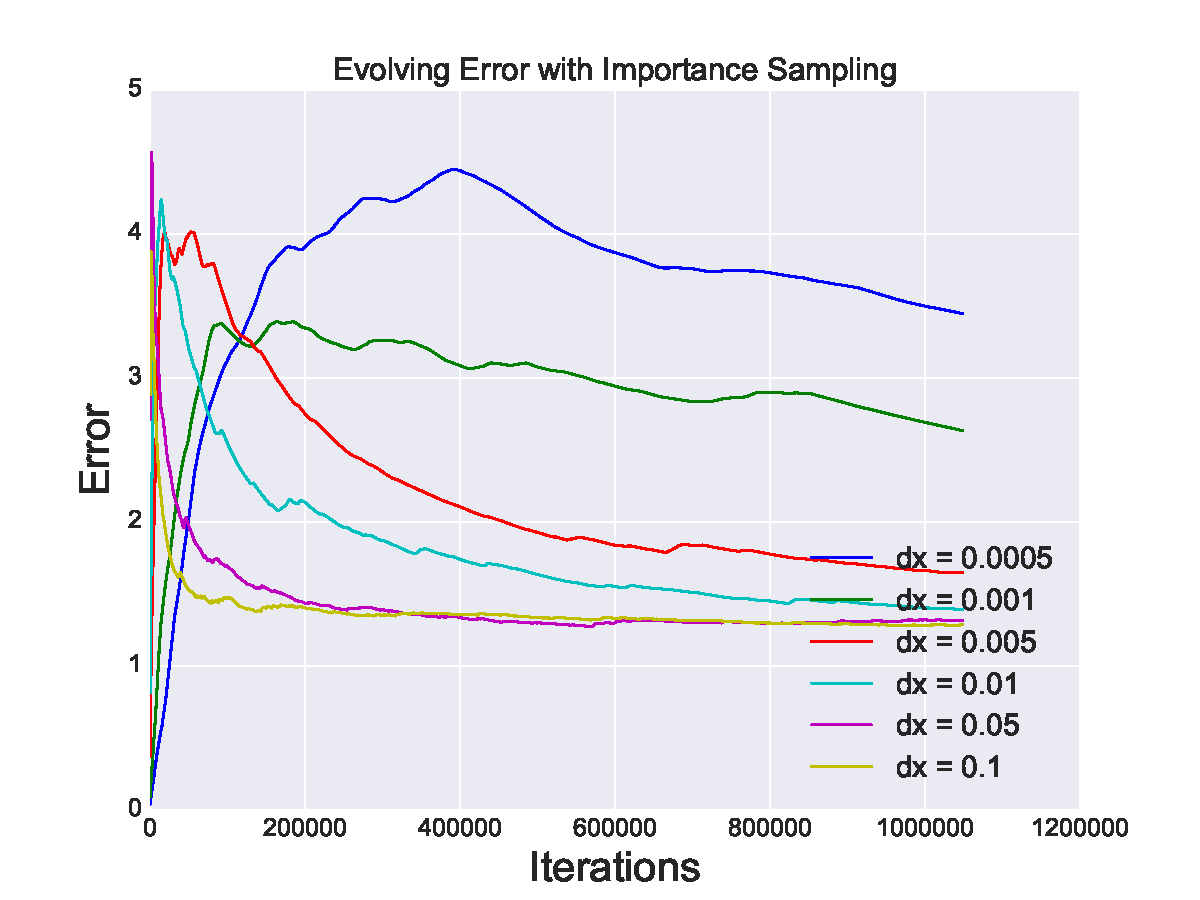
\includegraphics[width=.8\linewidth]{../Results/EvoStdIS.pdf}
				\caption{Standard deviation of the energy}
			\end{subfigure}
			\caption{Mean energy and standard deviation of the energy as a function of Monte Carlo cycles for various step sizes, $dx$. This was done with importance sampling in three dimensions, using $N=100$, $a=0$ (noninteracting), $\alpha=0.45$, $\omega_z=1$, $\beta=1$,}\label{fig:find_dx_importance}
		\end{figure}
	As explained in section \textbf{SECTION}, we choose $dt=0.05$.
	\subsection{Testing our code}
	We test our code by running the simulations for the noninteracting case ($a=0$) and for the correct value of the variational parameter, $\alpha=0.5$. We then expect our code to reproduce the exact energy given in equation \ref{eq:Exact_Energy_N_particles}. We test this using both the analytic and the numeric energy, and time the CPU difference between them.  We compute the uncertainty using the blocking method, as described in section \ref{sec:Blocking}. We show the results without importance sampling in table \ref{tab:4.1_benchmark_no_Green} (1D), table \ref{tab:4.1_benchmark_no_Green_2D} (2D)  and table \ref{tab:4.1_benchmark_no_Green_3D} (3D).
	\begin{table}[ht!]
		\begin{adjustwidth}{-2cm}{}
			\begin{tabular}{cccccc}
				N & Analytic energy, $E_a$ [$\hbar \omega$] & Numeric energy, $E_n$ [$\hbar \omega$] & Exact energy, $E$ [$\hbar \omega$]& CPU time $E_a$ [s] &CPU time $E_n$ [s]\\
				\hline
				1&$0.5$&$0.5$&$0.5$& 1.41&2.03\\
				10&$5$&$5.00000\pm 1\cdot 10^{-5}$&$5$& $1.47$&9.13\\
				100&$50$&$50.000\pm 0.001$&$50$&2.42&446.83\\
				500&$250$&-&250 &51.02 &-
			\end{tabular}
		\end{adjustwidth}
		\caption{Benchmarking of our code in the noninteracting case ($a=0$), in one dimension, showing the analytic energy (computed by means of equation \ref{eq:Local_energy_all}), the numeric energy and the exact energy (given by equation \ref{eq:Exact_Energy_N_particles}). This is for the spherical trap ($\omega_z=\beta=1$) in one dimension. This was obtained using $4$ cores, each running $2^{20}$ Monte Carlo cycles. The simulation with the numeric energy for $N=500$ took too long to be feasible. Wherever no uncertainty is specified, blocking gave an error of $0$. This is with brute force sampling.}\label{tab:4.1_benchmark_no_Green}
	\end{table}
	\begin{table}[ht!]
		\begin{adjustwidth}{-2cm}{}
			\begin{tabular}{cccccc}
				N & Analytic energy, $E_a$ [$\hbar \omega$] & Numeric energy, $E_n$ [$\hbar \omega$] & Exact energy, $E$ [$\hbar \omega$]& CPU time $E_a$ [s] &CPU time $E_n$ [s]\\
				\hline
				1&$1$&$1$&$1$& 1.32&2.27\\
				10&$10$&$10.00000\pm 3\cdot 10^{-5}$&$10$& $1.49$&15.11\\
				100&$100$&$100.000\pm 0.003$&$50$&2.65&810.2\\
				500&$500$&- &$500$&49.2 &-
			\end{tabular}
		\end{adjustwidth}
		\caption{Same table as table \ref{tab:4.1_benchmark_no_Green}, but in 2 dimensions}\label{tab:4.1_benchmark_no_Green_2D}
	\end{table}
		\begin{table}[ht!]
			\begin{adjustwidth}{-2cm}{}
				\begin{tabular}{cccccc}
					N & Analytic energy, $E_a$ [$\hbar \omega$] & Numeric energy, $E_n$ [$\hbar \omega$] & Exact energy, $E$ [$\hbar \omega$]& CPU time $E_a$ [s] &CPU time $E_n$ [s]\\
					\hline
					1&$1.5$&$1.5$&$1.5$& 1.56&2.85\\
					10&$15$&$15.00000\pm 6\cdot 10^{-5}$&$15$& $1.91$&29.89\\
					100&$150$&$149.997\pm 0.005$&$150$&3.92&1791.83\\
					500&$750$&- &$750$&54.36 &-
				\end{tabular}
			\end{adjustwidth}
			\caption{Same table as table \ref{tab:4.1_benchmark_no_Green}, but in 3 dimensions}\label{tab:4.1_benchmark_no_Green_3D}
		\end{table}
		We do a similar analysis with importance sampling. This gives table \ref{tab:4.1_benchmark_Green} (1D), table \ref{tab:4.1_benchmark_Green_2D} (2D) and table \ref{tab:4.1_benchmark_Green_3D} (3D).
		 \begin{table}[ht!]
			\begin{adjustwidth}{-2cm}{}
				\begin{tabular}{cccccc}
					N & Analytic energy, $E_a$ [$\hbar \omega$] & Numeric energy, $E_n$ [$\hbar \omega$] & Exact energy, $E$ [$\hbar \omega$]& CPU time $E_a$ [s] &CPU time $E_n$ [s]\\
					\hline
					1&$0.5$&$0.5$&$0.5$& 1.83&2.36\\
					10&$5$&$5.00000\pm 2\cdot 10^{-5}$&$5$& $2.03$&9.59\\
					100&$50$&$49.997\pm 0.001$&$50$&4.92&441.62\\
					500&$250$&-&250 &56.83 &-
				\end{tabular}
			\end{adjustwidth}
			\caption{Benchmarking of our code in the noninteracting case ($a=0$), in one dimension, showing the analytic energy (computed by means of equation \ref{eq:Local_energy_all}), the numeric energy and the exact energy (given by equation \ref{eq:Exact_Energy_N_particles}). This is for the spherical trap ($\omega=\omega_z=\beta=1$) in one dimension. This was obtained using $4$ cores, each running $2^{20}$ Monte Carlo cycles. The simulation with the numeric energy for $N=500$ took too long to be feasible. Wherever no uncertainty is specified, blocking gave an error of $0$. This is with importance sampling.}\label{tab:4.1_benchmark_Green}
		\end{table}
		 \begin{table}[ht!]
		 	\begin{adjustwidth}{-2cm}{}
		 		\begin{tabular}{cccccc}
		 			N & Analytic energy, $E_a$ [$\hbar \omega$] & Numeric energy, $E_n$ [$\hbar \omega$] & Exact energy, $E$ [$\hbar \omega$]& CPU time $E_a$ [s] &CPU time $E_n$ [s]\\
		 			\hline
		 			1&$1$&$1$&$1$& 1.87&2.80\\
		 			10&$10$&$10.00004\pm 3\cdot 10^{-5}$&$10$& $2.16$&16.86\\
		 			100&$100$&$99.998\pm 0.003$&$100$&5.71&808.74\\
		 			500&$500$&-&500 &58.17 &-
		 		\end{tabular}
		 	\end{adjustwidth}
		 	\caption{Same as table \ref{tab:4.1_benchmark_Green} but in 2 dimensions.}\label{tab:4.1_benchmark_Green_2D}
		 \end{table}
		 \begin{table}[ht!]
		 	\begin{adjustwidth}{-2cm}{}
		 		\begin{tabular}{cccccc}
		 			N & Analytic energy, $E_a$ [$\hbar \omega$] & Numeric energy, $E_n$ [$\hbar \omega$] & Exact energy, $E$ [$\hbar \omega$]& CPU time $E_a$ [s] &CPU time $E_n$ [s]\\
		 			\hline
		 			1&$1.5$&$1.5$&$1.5$& 1.87&3.08\\
		 			10&$15$&$14.99999\pm 6\cdot 10^{-5}$&$15$& $2.66$&26.26\\
		 			100&$150$&$149.997\pm 0.006$&$150$&6.40&1672.32\\
		 			500&$750$&-&750 &58.55 &-
		 		\end{tabular}
		 	\end{adjustwidth}
		 	\caption{Same as table \ref{tab:4.1_benchmark_Green} but in 3 dimensions.}\label{tab:4.1_benchmark_Green_3D}
		 \end{table}
	As discussed further in section \textbf{SECTION}, we opt to not use importance sampling in the interacting case.
	\subsection{Energy as a function of $\boldsymbol{\alpha}$}
	To investigate how our solution varies with $\alpha$, we plot the local energy as a function of the variational parameter $\alpha$. We first do this for the spherical harmonic oscillator ($\beta=1$) with no interaction ($a=0$), with $N=100$ and $2^{20}$ Monte Carlo cycles per core (running with $4$ cores). We also compute the error in each case, using the blocking method. This gives the plot shown in figure \ref{fig:Average_EL_N=100_brute_force} (brute-force sampling) and figure \ref{fig:Average_EL_N=100_importance} (importance sampling).
	\begin{figure}[ht!]
		\centering
		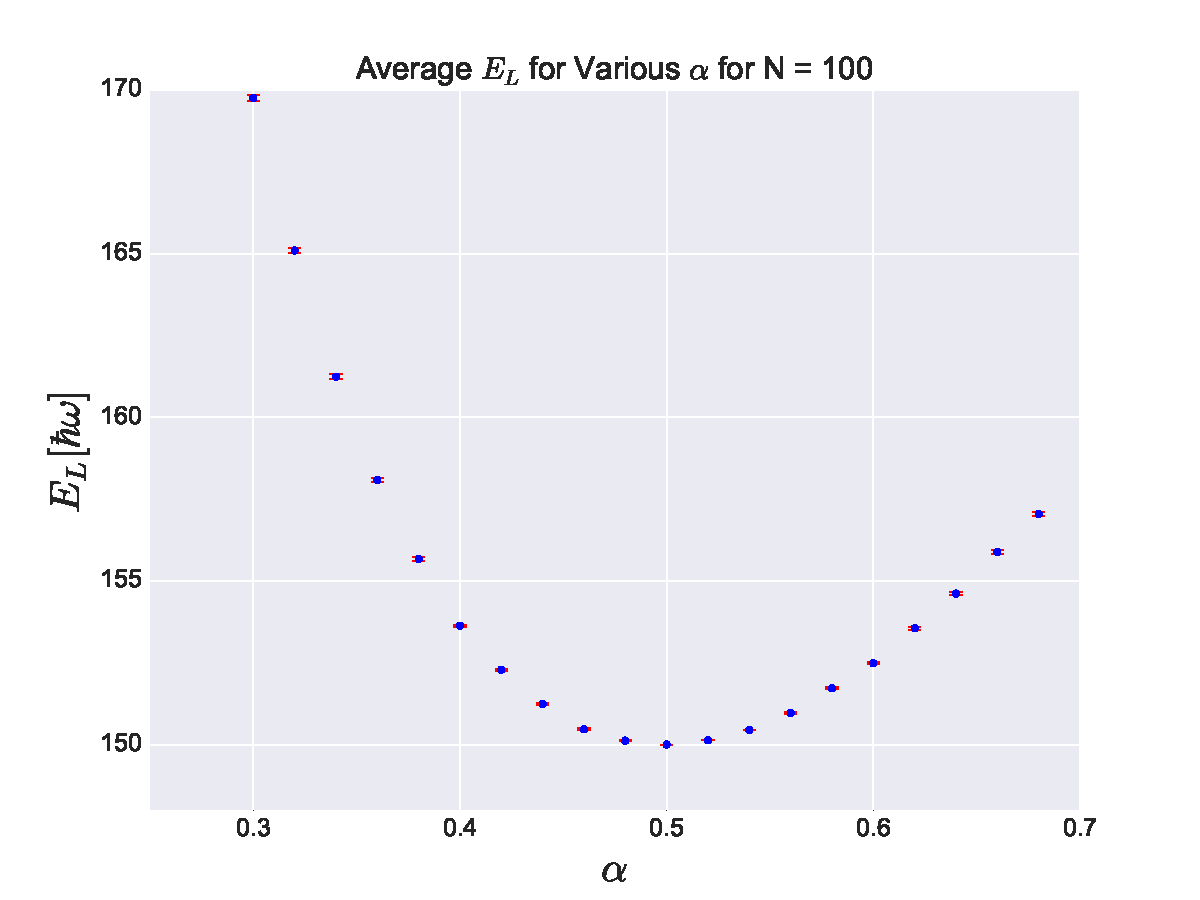
\includegraphics[scale=0.8]{../Results/N100ax20/EvAlphaN100.pdf}
		\caption{Local energy for various values of $\alpha$, for $a=0$, $\beta=1$, $\omega_z=1$, $N=100$, 3 dimensions, $2^{20}$ Monte Carlo cycles and brute force sampling.}\label{fig:Average_EL_N=100_brute_force}
	\end{figure}	
		\begin{figure}[ht!]
			\centering
			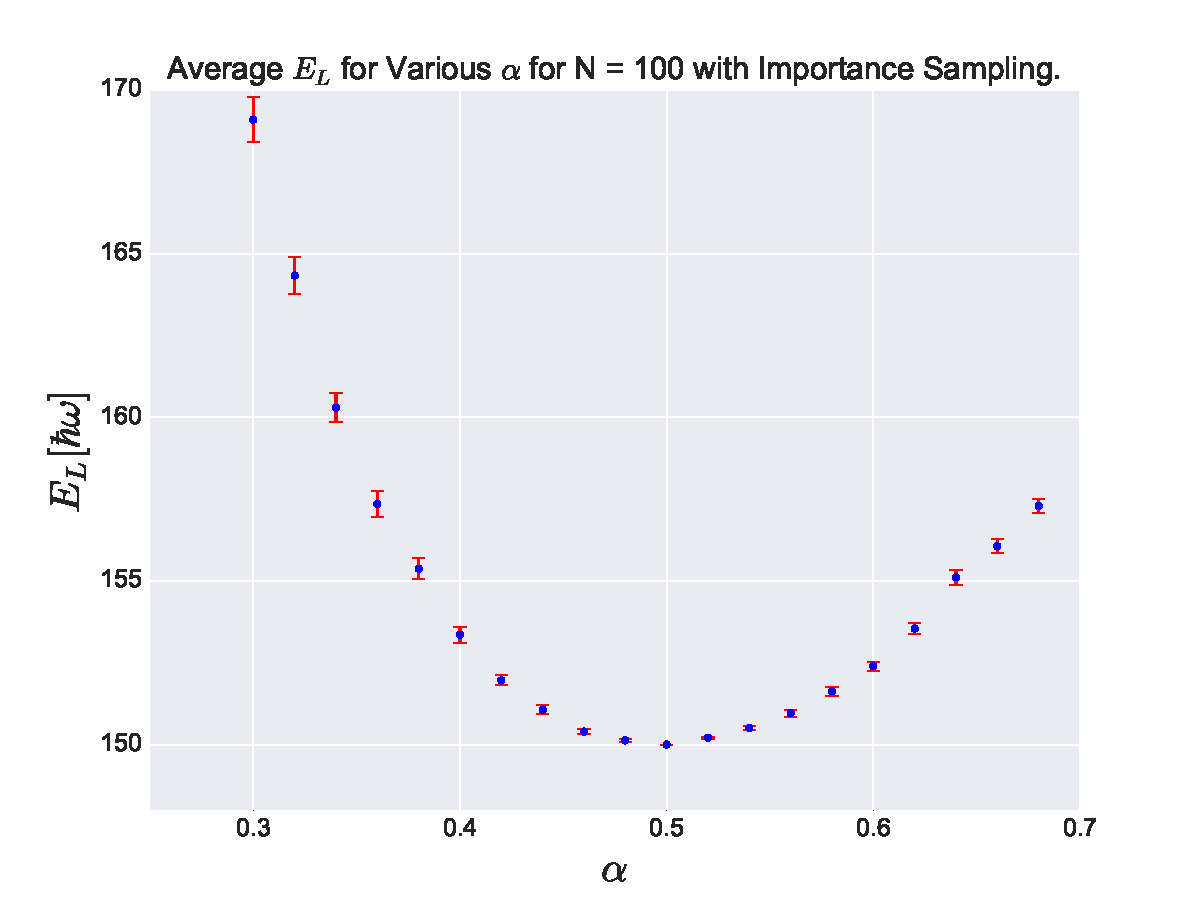
\includegraphics[scale=0.8]{../Results/N100ax20/EvAlphaN100IS.pdf}
			\caption{Local energy for various values of $\alpha$, for $a=0$, $\beta=1$, $\omega_z=1$, $N=100$, 3 dimensions, $2^{20}$ Monte Carlo cycles and importance sampling.}\label{fig:Average_EL_N=100_importance}
		\end{figure}
	We do a similar analysis for $N=10$ in the interacting case\footnote{Any higher $N$ was far too slow.}. This gives the plot shown in figure \ref{fig:EL_alpha_N10_interacting} for brute-force sampling.
			\begin{figure}[ht!]
				\centering
				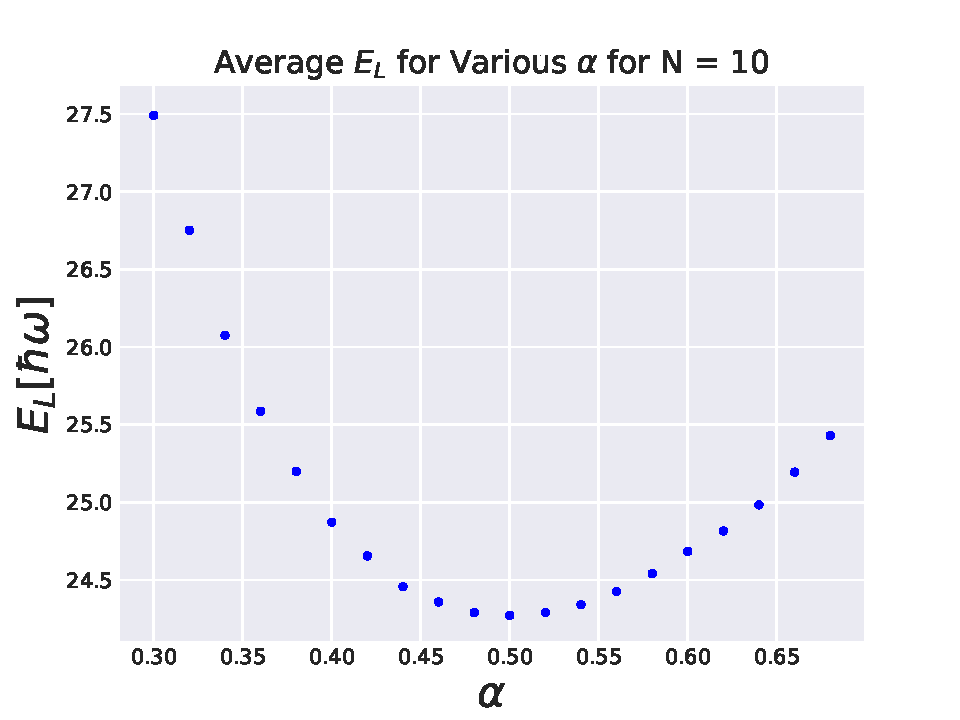
\includegraphics[scale=0.8]{../Results/Alpha_v_EL_Interacting_N10.pdf}
				\caption{Local energy for various values of $\alpha$, for $a=0.0043$, $\omega=1$, $\omega_z=\beta=2.82843$, $N=10$, 3 dimensions, $2^{20}$ Monte Carlo cycles and brute force sampling. The error bars are too small to be shown.}\label{fig:EL_alpha_N10_interacting}
			\end{figure}
	\subsection{Finding the optimal $\boldsymbol{\alpha}$}
	We run our gradient descent method for various $N$ in the fully interacting case, to find the optimal parameter. We first test our method by running it for the 3D noninteracting system of $10$ particles, and ensuring that it finds the correct value at $\alpha=0.5$. The result of this is shown in figure \ref{fig:gradient_descent_noninteracting}.
			\begin{figure}[ht!]
				\centering
				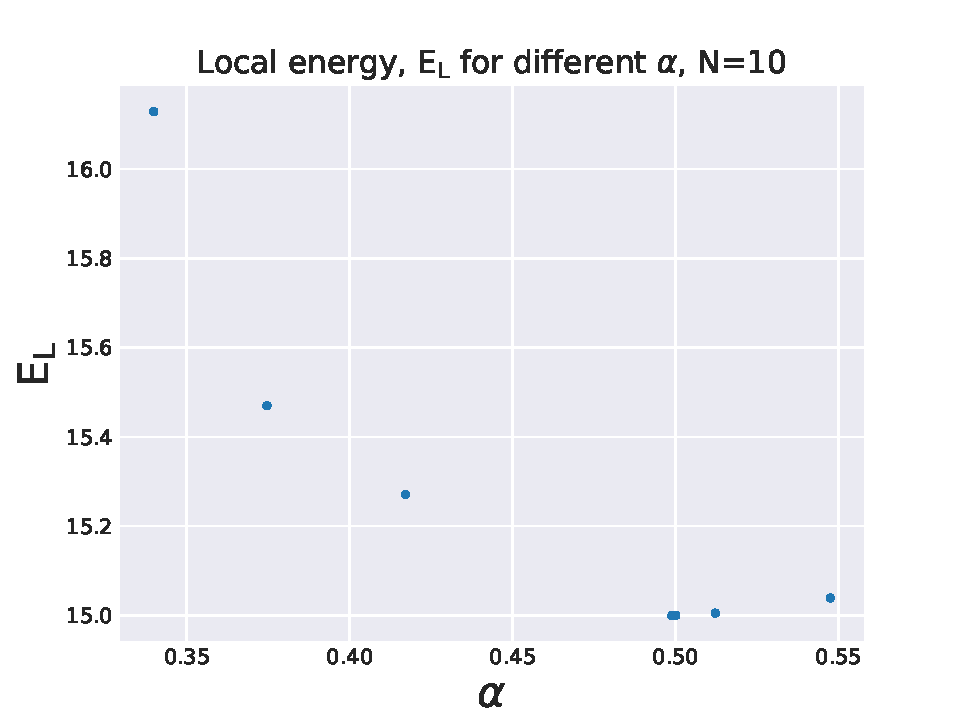
\includegraphics[scale=0.8]{../Results/E_v_alpha_gradient_noninteracting.pdf}
				\caption{Gradient descent for finding the optimal $\alpha$ in the noninteracting case ($a=0$), with $N=10$, $\omega=\omega_z=\beta=1$, 3 dimensions and brute-force sampling. We use a minimum step size, $\epsilon=10^{-6}$, and an accept whenever the gradient is less than $10^{-6}$.}\label{fig:gradient_descent_noninteracting}
			\end{figure}
	The method finds $\alpha=0.5$ in few time steps. We do a similar analysis for the interacting case with $N=10,50$ and $100$. This is shown in figure \ref{fig:gradient_descent_interactingN10} (N=10), figure \ref{fig:gradient_descent_interactingN50} (N=50).
		\begin{figure}[ht!]
			\centering
			\centering
			\begin{subfigure}{.5\textwidth}
				\centering
				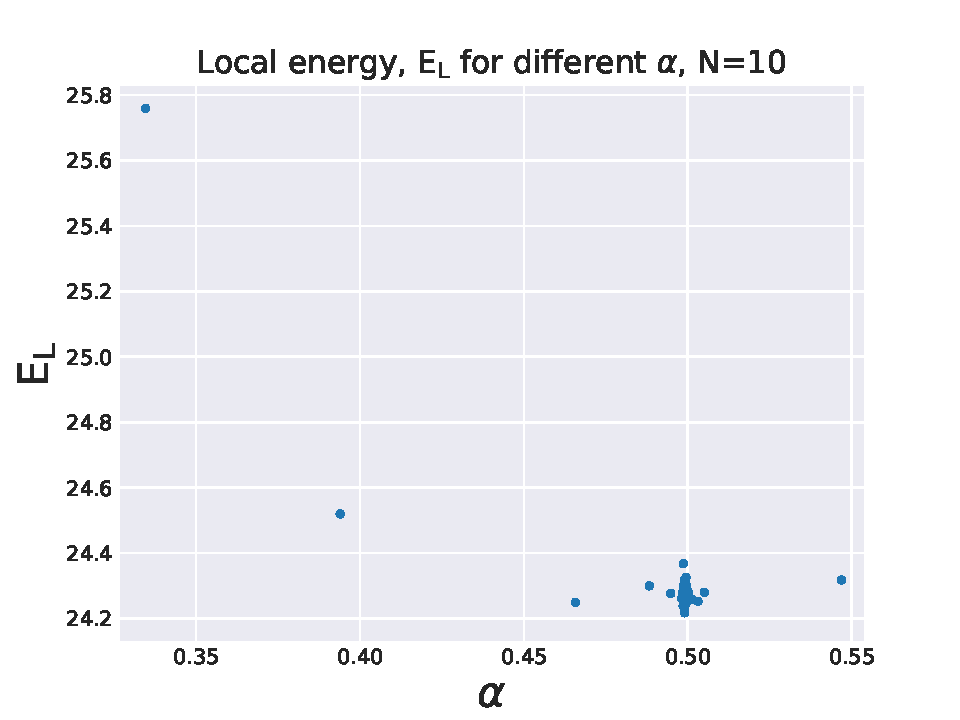
\includegraphics[width=.8\linewidth]{../Results/E_v_alpha_gradient.pdf}
				\caption{Gradient descent}
			\end{subfigure}%
			\begin{subfigure}{.5\textwidth}
				\centering
				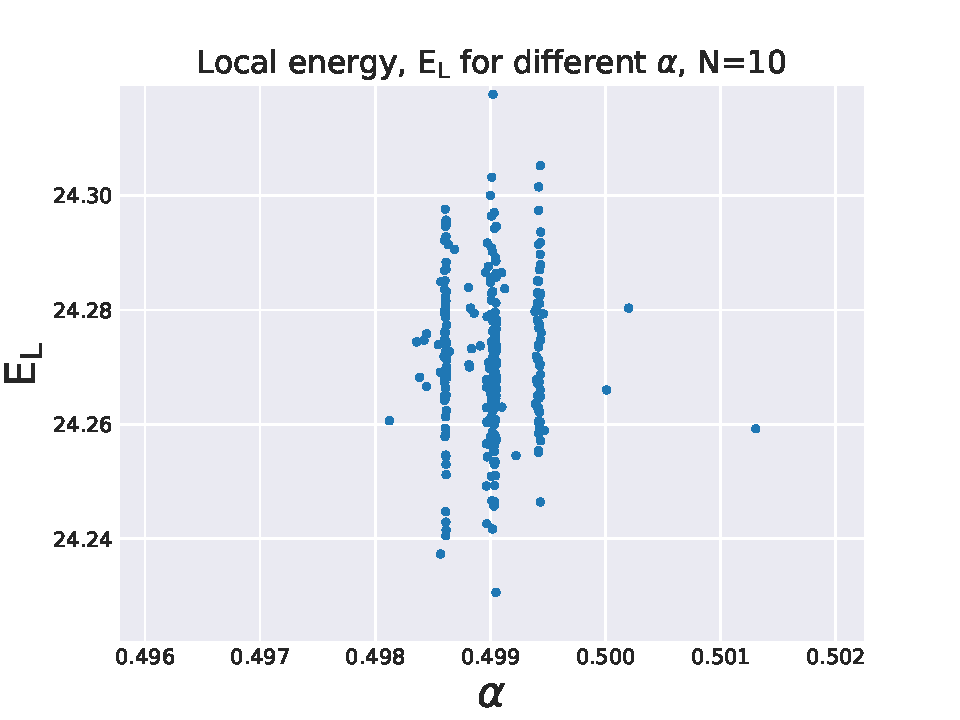
\includegraphics[width=.8\linewidth]{../Results/E_v_alpha_gradient_zoom.pdf}
				\caption{Zoomed in version}
			\end{subfigure}
			\caption{Gradient descent for finding the optimal $\alpha$ in the interacting case ($a=0.0043$), with $N=10$, $\omega=1$, $\omega_z=\beta=2.82843$, 3 dimensions and brute-force sampling. We use a minimum step size, $\epsilon=10^{-6}$, and an accept whenever the gradient is less than $10^{-6}$. We show also a zoomed-in version of the same plot.}\label{fig:gradient_descent_interactingN10}
		\end{figure}
				\begin{figure}[ht!]
					\centering
					\centering
					\begin{subfigure}{.5\textwidth}
						\centering
						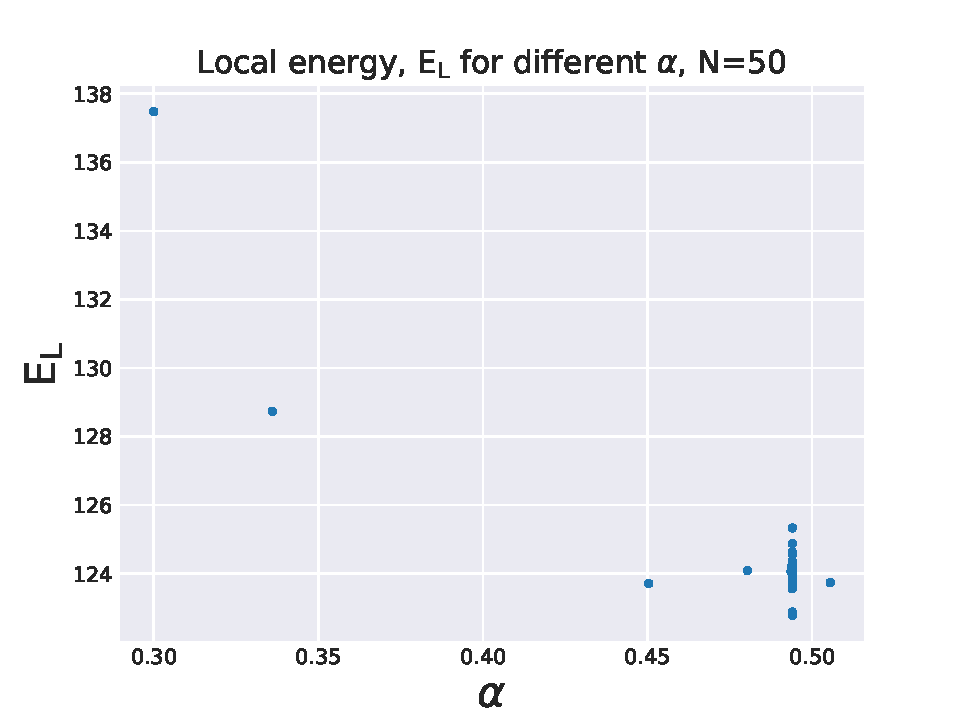
\includegraphics[width=.8\linewidth]{../Results/E_v_alpha_gradientN50.pdf}
						\caption{Gradient descent}
					\end{subfigure}%
					\begin{subfigure}{.5\textwidth}
						\centering
						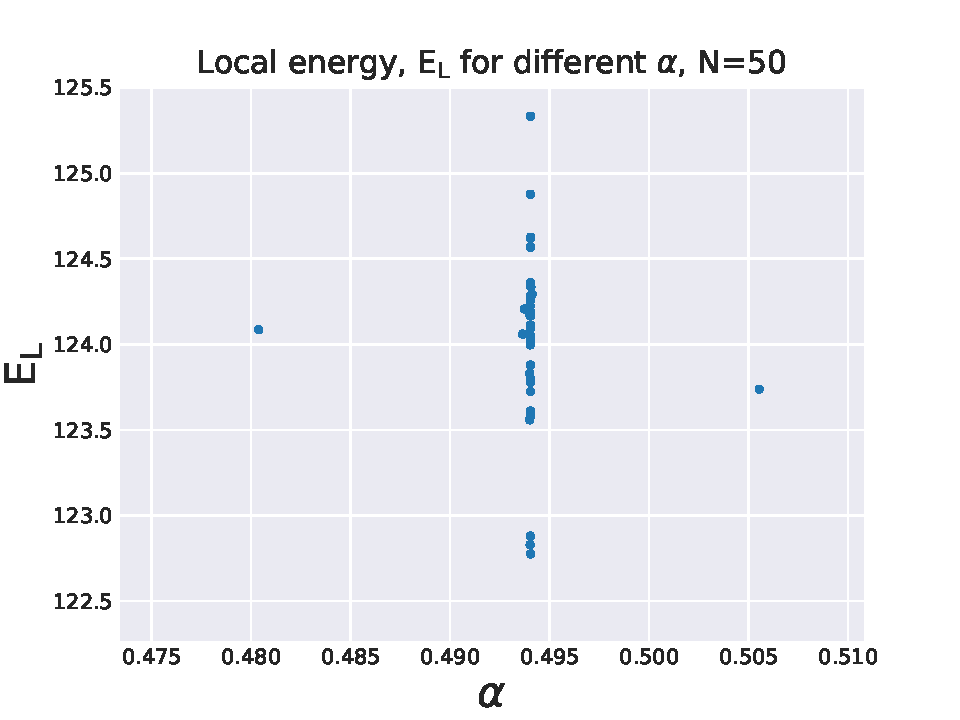
\includegraphics[width=.8\linewidth]{../Results/E_v_alpha_gradientN50Zoom.pdf}
						\caption{Zoomed in version}
					\end{subfigure}
					\caption{Same as figure \ref{fig:gradient_descent_interactingN10} but with $N=50$. }\label{fig:gradient_descent_interactingN50}
				\end{figure}
		
			\begin{table}[ht!]
				\centering
				\begin{tabular}{cccc}
					N & $\alpha$\\
					\hline
					10 & $0.499037$\\
					50 &$0.494033$\\ 
					100 & 
				\end{tabular}
				\caption{Values for the variational parameter $\alpha$ for various $N$. This was estimated in 3 dimensions, with $a=0.0043$, $\omega=1$, $\omega_z=\beta=2.82843$ and using brute force sampling with $2^{20}/100$ timesteps. We stopped the gradient descent method once it became stable, but after a minimum of $40$ iterations.}\label{tab:correct_alpha_interacting}
		\end{table}
	\subsection{Results from the fully interacting system}
	We now run the fully interacting system. We choose the parameters used by \cite{Nilsen2005}, and an $\alpha$ value found by the gradient descent. We do not use importance sampling, as it took too long. We use the analytic expression for the local energy, given in equation \ref{eq:Local_energy_all}. This gives the values shown in table \ref{tab:fully_interacting_system}.
	\begin{table}[ht!]
		\centering
		\begin{tabular}{cccc}
			N & Local energy, $E_L$ [$\hbar \omega$] & CPU time [s]\\
			\hline
			10 & $24.14259\pm 9\cdot 10^{-5}$ & 78.4679\\
			50 & $123.859\pm 0.001$ & 4338.12\\
			100 & $253.12 \pm 0.06$ & 31442.4\\
		\end{tabular}
		\caption{Local energy in 3 dimensions for the fully interacting system. We use the parameters used by \cite{Nilsen2005}, i.e. $a=0.0043$, $\omega_z=\beta=2.82843$, $\omega=1$. We use brute force sampling, and the parameters $\alpha$ found by our gradient descent method, shown in table \ref{tab:correct_alpha_interacting}.}\label{tab:fully_interacting_system}
	\end{table}
	\subsection{Onebody densities}
	We plot the onebody density for the interacting and noninteracting case in figure \ref{fig:results_onebody} below.
		\begin{figure}[ht!]
			\centering
			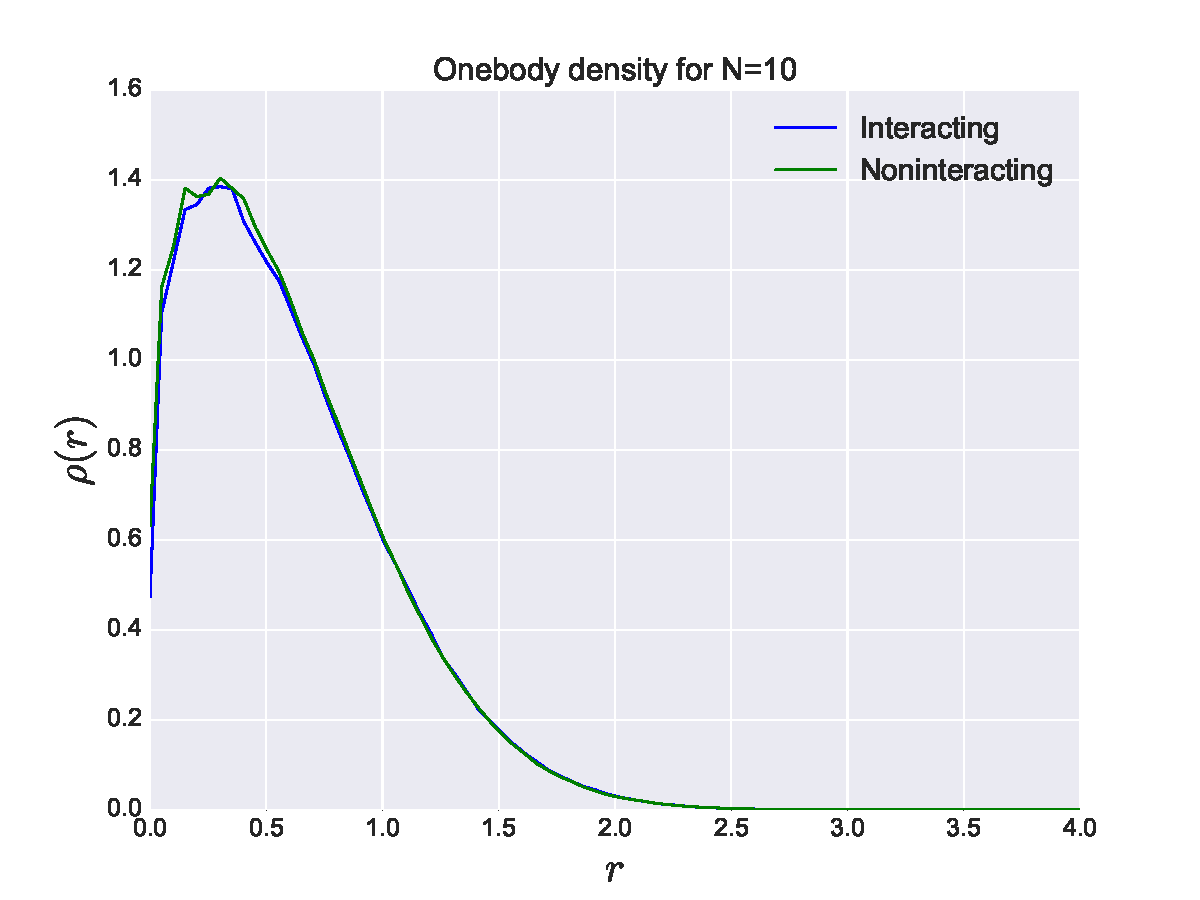
\includegraphics[scale=0.8]{../Results/onbody.pdf}
			\caption{Radial onebody density for noninteracting ($a=0$) and interacting ($a=0.0043$), using $\omega_z=\omega=\beta=1$, $N=10$ particles in $3$ dimensions and using brute force sampling.}\label{fig:results_onebody}
		\end{figure}
	\section{Discussion}
	
	\section{Conclusion}
	
	\subsection{Conclusion}
	
	\subsection{Outlook}
	\bibliographystyle{apalike}
	\bibliography{Project1}
	\begin{appendices}
		\section{Analytic expression for the local energy and quantum force}\label{ap:analytic_expression_for_the_local_energy_and_quantum_force}
		\paragraph{First derivative:}
		For particle $k$, $\nabla_k$ is given by:
		\begin{equation}
		\nabla_k\Psi_{T} = \nabla_k\left(\Psi_T(\mathbf{r})=\nabla_k \prod_{i=1}^n\phi(\mathbf{r}_i)\exp\left(\sum_{i<j} u(r_{ij})\right)\right)
		\end{equation}
		Now apply the product rule. For the first term, all terms are unchanged except where $i=k$, giving the first term as:
		\begin{equation}
		\nabla_k \phi(\mathbf{r}_k)\left[ \prod_{i\neq k} \phi(\mathbf{r}_i)\right]\exp\left(\sum_{i<j}u(r_{ij})\right)
		\end{equation}
		The second term is trickier. We can rewrite it as follows:
		\begin{align}
		\prod_{i}\phi(\boldsymbol{r}_{i})\nabla_{k}\left[\exp\left(\sum_{i < j}u(r_{ij})\right)\right]
		= \prod_{i}\phi(\boldsymbol{r}_{i})\nabla_{k}\left[\exp\left(\sum_{j = 1}^{n}\sum_{i = 1}^{j-1}u(r_{ij})\right)\right]
		\label{second term in first derivative}
		\end{align}
		This is calculated by using the chain-rule. To evaluate the innerfunction, we must look
		at \\$1 \le j \le k$, $j = k$ and $j \ge k$. Begining with $1\le  j \le k$,
		the first sum is from $1$ up the kth particle, meaning all terms differentiated before $k$ vanishes
		and we are left with $u(r_{ik})$, thus leaving with us with:
		\begin{align}
		\prod_{i}\phi(\boldsymbol{r}_{i})\nabla_{k}\left[\exp\left(\sum_{j = 1}^{k}\sum_{i = 1}^{k-1}u(r_{ij})\right)\right]
		=
		\prod_{i}\phi(\boldsymbol{r}_{i})\exp{\left(\sum_{i<j}u(r_{ij})\right)}
		\left[\sum_{i = 1}^{k-1}\nabla_{k}u(r_{ik})\right]
		\end{align}
		For $j = k$, we see that the first sum goes from and end up at kth particle, meaning
		this sum vanishes, secondly, the second sum is evaluated at $1 \le i \le k-1$, leaving with
		constants up to $k-1$, thus this term becomes $0$.
		\begin{align}
		\prod_{i}\phi(\boldsymbol{r}_{i})\nabla_{k}\left[\exp\left(\sum_{j = 1}^{n}\sum_{i = 1}^{j-1}u(r_{ij})\right)\right]
		= 0
		\end{align}
		For $j > k$,the first sum goes from $k+1\le j \le n$ and the second $1 \le i \le k$.  The second sum vanishes, because all constants are differentiated away
		except the last term $i = k$. This leaves us with:
		\begin{align}
		\prod_{i}\phi(\boldsymbol{r}_{i})\nabla_{k}\left[\exp\left(\sum_{j = k+1}^{n}\sum_{i = 1}^{k}u(r_{ij})\right)\right]
		= \prod_{i}\phi(\boldsymbol{r}_{i})
		\exp{\left(\sum_{i<j}u(r_{ij})\right)}
		\left[\sum_{j = k + 1}^{n}\nabla_{k}u(r_{kj})\right]
		\end{align}
		We can now write the second term as \ref{second term in first derivative}):
		\begin{align}\label{combined sum}
		\prod_{i}\phi(\boldsymbol{r}_{i})
		\exp{\left(\sum_{i<j}u(r_{ij})\right)}
		\left[\sum_{j = k + 1}^{n}\nabla_{k}u(r_{kj}) +
		\left[\sum_{i = 1}^{k-1}\nabla_{k}u(r_{ik})\right]\right]
		\end{align}
		%CHECK THIS EQUATION
		This can be rewritten to:
		\begin{align}
		\prod_{i}\phi(\boldsymbol{r}_{i})
		\exp{\left(\sum_{i<j}u(r_{ij})\right)}
		\left[\sum_{j \neq k}\nabla_{k}u(r_{kj})\right]
		\end{align}
		Thus the first derivative of the trial wavefunction
		can be written as:
		\begin{align}
		\nabla_{k}\Psi_{T} =
		\nabla_k \phi(\mathbf{r}_k)\left[ \prod_{i\neq k} \phi(\mathbf{r}_i)\right]\exp\left(\sum_{i<j}u(r_{ij})\right)
		+ \prod_{i}\phi(\boldsymbol{r}_{i})
		\exp{\left(\sum_{i<j}u(r_{ij})\right)}
		\left[\sum_{j \neq k}u(r_{kj})\right]
		\end{align}
		\paragraph{Second derivative:}
		Lastly we will calculate the second derivative of the trial function, where we
		use the product rule and the chain rule. We will then obtain the following:
		\begin{align*}
		\begin{split}
		\nabla_{k}^2\Psi_{T} =
		\underbrace{\nabla_k^2 \phi(\mathbf{r}_k)\left[ \prod_{i\neq k} \phi(\mathbf{r}_i)\right]\exp\left(\sum_{i<j}u(r_{ij})\right)}_{\mathrm{I}} +\\
		\underbrace{2\left(\nabla_k \phi(\mathbf{r}_k)\left[ \prod_{i\neq k} \phi(\mathbf{r}_i)\right]
			\exp{\left(\sum_{i<j}u(r_{ij})\right)}
			\left[\sum_{j \neq k}\nabla_{k}u(r_{kj})\right]\right)}_{\mathrm{II}} +
		\\
		\underbrace{\prod_{i}\phi(\boldsymbol{r}_{i})
			\exp{\left(\sum_{i<j}u(r_{ij})\right)}
			\left[\sum_{j \neq k}\nabla_{k}u(r_{kj})\right]^2}_{\mathrm{III}} +
		\\
		\underbrace{\prod_{i}\phi(\boldsymbol{r}_{i})
			\exp{\left(\sum_{i<j}u(r_{ij})\right)}
			\left[\sum_{j \neq k}\nabla_{k}\nabla_{k}u(r_{kj})\right]}_{\mathrm{IV}}
		\end{split}
		\end{align*}
		Where the derivatives of the different parts are obtained from previous.
		We will now divide the second derivative by the trial wavefunction, and obtain:
		\begin{align}
		\frac{1}{\Psi_{T}}\nabla_{k}^2\Psi_{T} =
		\underbrace{\frac{\nabla_{k}^2\phi{(\boldsymbol{r}_{k})}}{\phi(\boldsymbol{r}_{\phi(\boldsymbol{r}_{k})})}}_{\mathrm{I}}
		+ \underbrace{2\frac{\nabla_{k}\phi(\boldsymbol{r}_{k})}{\phi{(\boldsymbol{r}_{k})}}\sum_{j\neq k}\nabla_{k}u(r_{kj})}_{\mathrm{II}}
		+ \underbrace{\left(\sum_{j\neq k}\nabla_{k} u(r_{kj})\right)^2}_{\mathrm{III}} +
		\underbrace{\left[\sum_{j \neq k}\nabla_{k}\nabla_{k}u(r_{kj})\right]}_{\mathrm{IV}}
		\end{align}
		We will now carry out the differentiation in term (II), (III) and (IV). Begining with the
		(II), by using the chain rule we can rewrite (II) as:
		\begin{align*}
		2\frac{\nabla_{k}\phi(\boldsymbol{r}_{k})}{\phi{(\boldsymbol{r}_{k})}}\sum_{j\neq k}\pdv{u(r_{kj})}{r_{kj}}\pdv{r_{kj}}{\boldsymbol{r}_{k}} =
		2\frac{\nabla_{k}\phi(\boldsymbol{r}_{k})}{\phi{(\boldsymbol{r}_{k})}}\left(\sum_{j\neq k}\frac{\boldsymbol{r}_{k} - \boldsymbol{r}_{j}}{r_{kj}}u'(r_{kj})\right)
		\end{align*}
		Where we have used $\nabla_{k} r_{kj} = (\boldsymbol{r}_{k} - \boldsymbol{r}_{j})/r_{kj}$.
		Looking at (III), we can write out the square into two factors. The second paranthese the summation index is replaced by a
		dummy index $i$. Thus will look as:
		\begin{align}
		\left(\sum_{j\neq k}\nabla_{k} u(r_{kj})\right)^2 = \left(\sum_{j\neq k}\nabla_{k} u(r_{kj})\right)\left(\sum_{i\neq k}\nabla_{k} u(r_{ki})\right)
		\end{align}
		From (II) we found the derivative of this function. Thus this can be expressed as (combining also the double sum):
		\begin{align}
		\left(\sum_{j\neq k}\nabla_{k} u(r_{kj})\right)^2 =
		\sum_{i, j\neq k}\left(\frac{\boldsymbol{r}_{k} - \boldsymbol{r}_{j}}{r_{kj}}\right)
		\left(\frac{\boldsymbol{r}_{k} - \boldsymbol{r}_{i}}{r_{ki}}\right)u'(r_{kj})u'(r_{ki})
		\end{align}
		The last part (IV), we must use the chain rule and product rule together. We will obtain
		the following term:
		\begin{align}
		\sum_{j \neq k}\nabla_{k}\nabla_{k}u(r_{kj}) =
		\sum_{j \neq k}\nabla_{k}\left(
		\left(\frac{\boldsymbol{r}_{k} - \boldsymbol{r}_{j}}{r_{kj}}\right)^2 u''(r_{kj}) + u'(r_{kj})\nabla_{k}
		\left(\frac{\boldsymbol{r}_{k} - \boldsymbol{r}_{j}}{r_{kj}}\right)\right)
		\end{align}
		Note that this is a unit vector squared:
		\begin{align}
		\left(\frac{\boldsymbol{r}_{k} - \boldsymbol{r}_{j}}{r_{kj}}\right)^2 = 1
		\end{align}
		and the last part is found by using the qoutient rule. This is the divergence to the vectors, since we are evaluating for
		specific particle k, and gradient to scalar (we must look for all combination of k particle):
		\begin{align}
		\nabla_{k}
		\left(\frac{\boldsymbol{r}_{k} - \boldsymbol{r}_{j}}{r_{kj}}\right)
		= \frac{r_{kj}\left(\nabla_{k}\cdot\boldsymbol{r}_{k}-
			\nabla_{k}\cdot\boldsymbol{r}_{j}\right) -
			(\boldsymbol{r}_{k}-\boldsymbol{r}_{j})\nabla_{k}r_{kj}}{r_{kj}^2}
		\end{align}
		This simply becomes:
		\begin{align}
		\nabla_{k}
		\left(\frac{\boldsymbol{r}_{k} - \boldsymbol{r}_{j}}{r_{kj}}\right)
		= \frac{3r_{kj}^2 - \boldsymbol{r}^2_{k} + 2(\boldsymbol{r}_{k}\cdot \boldsymbol{r}_{j}) - \boldsymbol{r}^2_{j}}{r_{kj}^3}
		\end{align}
		Note that $r_{kj} - \boldsymbol{r}^2_{k} + 2(\boldsymbol{r}_{k}\cdot \boldsymbol{r}_{j}) - \boldsymbol{r}^2_{j} = 0$, this leaves us with:
		\begin{align}
		\nabla_{k}
		\left(\frac{\boldsymbol{r}_{k} - \boldsymbol{r}_{j}}{r_{kj}}\right)
		= \frac{2}{r_{kj}}
		\end{align}
		Thus expression (IV) can be expressed as:
		\begin{align}
		\sum_{j \neq k}\nabla_{k}\nabla_{k}u(r_{kj}) =
		\sum_{j \neq k}\nabla_{k}\left(u''(r_{kj}) + \frac{2}{r_{kj}}u'(r_{kj})
		\right)
		\end{align}
		Combining (I), (II), (III) and (IV), we we will get that the second derivative
		of the trial function is:
		\begin{align}
		\begin{split}
		\frac{1}{\Psi_{T}}\nabla_{k}^2\Psi_{T} =
		\frac{\nabla_{k}^2\phi{(\boldsymbol{r}_{k})}}{\phi(\boldsymbol{r}_{k})}
		+
		2\frac{\nabla_{k}\phi(\boldsymbol{r}_{k})}{\phi{(\boldsymbol{r}_{k})}}\left(\sum_{j\neq k}\frac{\boldsymbol{r}_{k} - \boldsymbol{r}_{j}}{r_{kj}}u'(r_{kj})\right)
		+\\
		\sum_{i, j\neq k}\left(\frac{\boldsymbol{r}_{k} - \boldsymbol{r}_{j}}{r_{kj}}\right)
		\left(\frac{\boldsymbol{r}_{k} - \boldsymbol{r}_{i}}{r_{ki}}\right)u'(r_{kj})u'(r_{ki})
		+
		\sum_{j \neq k}\left(u''(r_{kj}) + \frac{2}{r_{kj}}u'(r_{kj})\right)
		\end{split}
		\end{align}
		\paragraph{Local energy:} Now that we have the second derivative of the
		trial-function, we can write out the analytical expression for the local energy.
		Recall that:
		\begin{align}
		E_{L}(\boldsymbol{r}) = \frac{1}{\Psi_{T}}H\Psi_{T} =
		\frac{1}{\Psi_{T}}\left[\sum_{i}^{N}\left(-\frac{\hbar^{2}}{2m}\nabla^{2}_{i}
		+ V_{ext}(\boldsymbol{r}_{i})\right) + \sum_{i < j}^{N}V_{int}(
		\boldsymbol{r}_{i},\boldsymbol{r}_{j})\right]\psi_{T}
		\end{align}
		The second derivative written explicitly is:
		\begin{align}
		\begin{split}
		\frac{1}{\Psi_{T}}\nabla^{2}_{k}\Psi_{T} = 4\alpha\boldsymbol{Q}_{k}^{2} - 4\alpha\boldsymbol{Q}_{k}
		\sum_{j\neq k}\left(\frac{\boldsymbol{r}_{k} - \boldsymbol{r}_{j}}{r_{kj}}u'(r_{kj})\right)
		+\\
		\sum_{i,j\neq k}\frac{\boldsymbol{r}_{k}\cdot\boldsymbol{r}_{k} - \boldsymbol{r}_{k}\cdot\boldsymbol{r}_{j} - \boldsymbol{r}_{k}\cdot\boldsymbol{r}_{i} + \boldsymbol{r}_{i}\cdot\boldsymbol{r}_{j}}{r_{kj}r_{ki}}u'(r_{ki})u'(r_{kj})
		\\
		+ \sum_{j \neq k}\left(u''(r_{kj}) + \frac{2}{r_{kj}}u'(r_{kj})\right)
		\end{split}
		\end{align}
		Where $\boldsymbol{Q}_{k} = \left(x_{k}\hat{i} + y_{k}\hat{j} + \beta z_{k}\hat{k}\right)$,
		and the first and second derivative of $u(r_{kj})$ is:
		\begin{align}
		u'(r_{kj}) =
		\begin{cases}
		\infty &, r_{kj} \le a\\
		\frac{a}{r_{kj}^{2} - ar_{kj}} &, r_{kj} > a
		\end{cases}
		\label{udiv}
		\end{align}
		and
		\begin{align}
		u''(r_{kj}) =
		\begin{cases}
		\infty &, r_{kj} \le a\\
		\frac{a^{2} - 2ar_{kj}}{\left(r_{kj}^{2} - ar_{kj}\right)^{2}} &, r_{kj} > a
		\end{cases}
		\label{udivdiv}
		\end{align}
		Thus the analytical local energy for a group of particle is:
		\begin{align}
		\begin{split}
		E_{L} = -\frac{\hbar^{2}}{2m}\sum_{k}\left[
		4\alpha^{2}\boldsymbol{Q}_{k}^{2} - 4\alpha\boldsymbol{Q}_{k} + \sum_{j \neq k}\left(\frac{\boldsymbol{r}_{k} - \boldsymbol{r}_{j}}{r_{kj}}u'(r_{kj})\right)\right.
		\\ \left. + \sum_{i,j \neq k}\left(\frac{\boldsymbol{r}\cdot\boldsymbol{r} + \boldsymbol{r}_{j}\cdot\boldsymbol{r}_{i} - \boldsymbol{r}_{j}\cdot\boldsymbol{r}_{k} -\boldsymbol{r}_{k}\cdot\boldsymbol{r}_{i}}{r_{ki}r_{kj}}u'(r_{ki})u'(r_{kj})\right)\right.
		\\
		\left. + \sum_{j \neq k}\left(u''(r_{kj} + \frac{2}{r_{kj}}u'(r_{kj}))\right)\right]
		+ \sum_{k}V_{ext}(\boldsymbol{r}_{k}) + \sum_{i < j}V_{int}(\boldsymbol{r}_{i}, \boldsymbol{r}_{j})
		\end{split}
		\end{align}
		This expression includes the situation where particles interact with each other.
		Now if we assume the particles does not interact with each other, we then have:
		\begin{align}
		E_{L} = \sum_{k}\left(4\alpha^{2}\boldsymbol{Q}_{k} + V_{ext}(\boldsymbol{r}_{k}) \right)
		\end{align}
		\paragraph{Quantum force/Drift force:}
		The quantum/drift force is defined to be:
		\begin{align}
		\boldsymbol{F}_{i} = 2\frac{\nabla\Psi_{T}}{\Psi_{T}}
		\end{align}
		Using the first derivative we just derived above this expression will look like:
		\begin{align}
		\boldsymbol{F}_{i} = 2\frac{\nabla_k \phi(\boldsymbol{r}_{k})}{\phi(\boldsymbol{r}_{k})}
		+
		2\sum_{j \neq k}\frac{\boldsymbol{r}_{k} - \boldsymbol{r}_{j}}{r_{kj}}u'(r_{kj})
		= -4\alpha\boldsymbol{Q}_{i} +
		2\sum_{j \neq k}\frac{\boldsymbol{r}_{k} - \boldsymbol{r}_{j}}{r_{kj}}u'(r_{kj})
		\end{align}
		Where $\boldsymbol{Q}_{i} = x_{i}\hat{i} + y_{i}\hat{j} + \beta z_{i}\hat{k}$ and
		$u'(r_{kj})$ is given in (\ref{udiv}). This is for a interacting case, since
		the distance between two particle and the gradient $kj$'th particle appears.
		Further notice that the quantum force can be written
		as $3\cross N$ matrix, where $N$ is number of particles in the system.
		For a non-interacting case, we have:
		\begin{align}
		\boldsymbol{F}_{i} = -4\alpha\boldsymbol{Q}_{i}
		\end{align}
		\section{The dimensionless Hamiltonian}\label{ap:dimensionless_hamiltonian}
		We aim to demonstrate that the Hamiltonian in equation \ref{eq:general_Hamiltonian} is equivalent to the Hamiltonian shown in equation \ref{eq:Hamiltonian_dimensionless} under the coordinate transformation:
		\begin{equation}
		\boldsymbol{r}\rightarrow \frac{\boldsymbol{r}}{a_{ho}}=\boldsymbol{r} \sqrt{\frac{m\omega}{\hbar}} \quad E\rightarrow \frac{E}{\hbar \omega}
		\end{equation}
		Where $a_{ho}=(h/m\omega)^{1/2}$. To show this, note first that the gradient operator under this transformation transforms as:
		\begin{equation}
		\nabla \rightarrow \sqrt{\frac{\hbar}{m\omega}} \nabla
		\end{equation}
		We now introduce this coordinate transformation into our Hamiltonian. This gives:
		\begin{equation}
		H\rightarrow H=\sum_{i=1}^{N}\left(-\frac{\hbar^2}{2m}\frac{\omega m}{\hbar}\nabla_i^2+\frac{1}{2}m\omega^2 \frac{\hbar}{m\omega}(x_i^2+y_i^2 +\omega_z^2 z_i^2) \right)+\sum_{i<j}^N V_{int}(\boldsymbol{r}_i, \boldsymbol{r}_j)
		\end{equation}
		Which can be rewritten as:
		\begin{equation}
		H=\frac{\hbar \omega}{2}\sum_{i=1}^N\left(-\nabla^2 +\frac{\hbar \omega}{2}\left(x_i^2+y_i^2 + \frac{\omega_z^2}{\omega^2}z_i^2\right)\right)+\sum_{i<j}^N V_{int}(\boldsymbol{r}_i, \boldsymbol{r}_j)
		\end{equation}
		Relabeling the energy and defining $\gamma=\omega_z/\omega$ gives:
		\begin{equation}
		H=\frac{1}{2}\sum_{i=1}^N \left(-\nabla_i^2 +x_i^2+y_i^2+\gamma z_i^2\right)+\sum_{i<j}^N V_{int}(\boldsymbol{r}_i, \boldsymbol{r}_j)
		\end{equation}
		Which is exactly equation \ref{eq:Hamiltonian_dimensionless}.
		
		\section{Deriving an approximate expression for the onebody density}\label{ap:approximte_onebody_density}
		We require that the spatial integral over the onebody density, $\rho(\boldsymbol{r_1})$ equals the total number of particles $N$. As we are only interested in the radial component of the onebody density, we consider only $\rho(r)$. This requirement can then be written as:
		\begin{equation}
		N=\int d^3 \boldsymbol{r} \rho(r)
		\end{equation} 
		Which gives, in spherical coordinates:
		\begin{equation}
		N=4\pi \int_0^{\infty}dr\  r^2 \rho(r)
		\end{equation}
		We now discretize this integral radius, choosing to integrate from $0$ to $r_{\mathrm{max}}$, where we choose $r_{\mathrm{max}}$ larger than the largest distance any particle deviates from the origin. This interval is divided into $M$ points, with a spacing of $\Delta r$. The discretized version of the integral then becomes:
		\begin{equation}
		N\approx 4\pi \sum_{i=1}^M r_i^2 \rho(r_i) \Delta r
		\end{equation}
		From which it follows that the onebody density can be computed as:
		\begin{equation}
		\rho(r_i)\approx \frac{N_i}{4\pi r_i^2 \Delta r}
		\end{equation}
		Where $N_i$ is the number of particles in the spherical shell with radius $r_i$ to $r_i+\Delta r$.
		
		\section{Finding the derivative of the local energy}\label{ap:derivative_of_local_energy}
		The local energy, $E_L$ is given by:
		\begin{equation}
		E_L=\langle \Psi_T | H| \Psi_T \rangle
		\end{equation}
We now want to find the derivative of the expectation value of the local energy $\langle E_{L}\rangle$
with respect to the variational parameter $\alpha$. Before we do that we must normalize the wavefunction:
\begin{align}
\ket{\Psi_{T}} = \frac{\ket{\Psi_{T}}}{\sqrt{\braket{\Psi_{T}}}}
\end{align}
The expectation value of the local energy is then:
\begin{align}
\langle E_{L} \rangle = \frac{\bra{\Psi_{T}}E_{L}\ket{\Psi_{T}}}{\braket{\Psi_{T}}}
\end{align}
Notice that can be written as:
\begin{align}
\langle E_{L} \rangle = \frac{\bra{\Psi_{T}}E_{L}\ket{\Psi_{T}}}{\braket{\Psi_{T}}}
= \frac{1}{\braket{\Psi_{T}}}\int..\int \Psi_{T}^{*}E_{L}\Psi_{T}\dd{\bold{r}_{1}}..\dd{\bold{r}_{N}}
\end{align}
Using the definition of $E_{L}$ and we know that the wavefunction is real, we get that:
\begin{align}
\langle E_{L} \rangle = \frac{1}{\braket{\Psi_{T}}}\int..\int \Psi_{T}^{*}\left(\frac{1}{\Psi_{T}}H\Psi_{T}\right)\Psi_{T}\dd{\bold{r}_{1}}..\dd{\bold{r}_{N}}
= \frac{1}{\braket{\Psi_{T}}}\int..\int H\Psi_{T}\Psi_{T}\dd{\bold{r}_{1}}..\dd{\bold{r}_{N}}
\end{align}
Thus this can be written as:
\begin{align}
\langle E_{L} \rangle = \frac{\bra{\Psi_{T}}H\ket{\Psi_{T}}}{\braket{\Psi_{T}}}
\end{align}
By using the product rule and differentiating this with respect to $\alpha$,
we will get:
\begin{align}
\pdv{\langle E_{L} \rangle }{\alpha} = \frac{1}{\braket{\Psi_{T}}}\pdv{\bra{\Psi_{T}}H\ket{\Psi_{T}}}{\alpha}
+ \bra{\Psi_{T}}H\ket{\Psi_{T}}\pdv{\alpha}\left(\frac{1}{\braket{\Psi_{T}}}\right)
\label{proddiff}
\end{align}
The first expression is:
\begin{align}
\frac{1}{\braket{\Psi_{T}}}\pdv{\bra{\Psi_{T}}H\ket{\Psi_{T}}}{\alpha}
=
\frac{1}{\braket{\Psi_{T}}}\pdv{\alpha}\int..\int\Psi_{T}^{*}H\Psi_{T}\dd{\bold{r}_{1}}..\dd{\bold{r}_{N}}
\end{align}
Taking the derivative into the integral and apply the product rule, we will obtain:
\begin{align}
\frac{1}{\braket{\Psi_{T}}}\int..\int\pdv{\Psi_{T}^{*}}{\alpha}H\Psi_{T}
+   \Psi_{T}^{*}\pdv{H}{\alpha}\Psi_{T}
+   \Psi_{T}^{*}H\pdv{\Psi_{T}}{\alpha}\dd{\bold{r}_{1}}..\dd{\bold{r}_{N}}
\end{align}
Since the hamiltonian does not depend on $\alpha$ we have:
\begin{align}
\frac{1}{\braket{\Psi_{T}}}\int..\int\underbrace{\pdv{\Psi_{T}^{*}}{\alpha}H\Psi_{T}}_{I}
+   \underbrace{\Psi_{T}^{*}H\pdv{\Psi_{T}}{\alpha}}_{II}\dd{\bold{r}_{1}}..\dd{\bold{r}_{N}}
\end{align}
We now wish to include the local energy in the integral, to do this we must
do some algebra. Consider the first expression ($I$):
\begin{align}
\frac{1}{\braket{\Psi_{T}}}\int..\int \pdv{\Psi_{T}^{*}}{\alpha}H\Psi_{T}\dd{\bold{r}_{1}}..\dd{\bold{r}_{N}}
\end{align}
By dividing and multiplying with $\Psi_{T}^{*}$ and $\Psi_{T}$ on the left and right for the
hamiltonian operator, we can write $I$ as:
\begin{align}
\begin{split}
\frac{1}{\braket{\Psi_{T}}}\int..\int \frac{\Psi_{T}^{*}}{\Psi_{T}^{*}}\pdv{\Psi_{T}^{*}}{\alpha}H\Psi_{T}\frac{\Psi_{T}}{\Psi_{T}}\dd{\bold{r}_{1}}..\dd{\bold{r}_{N}}
=
\\
\frac{1}{\braket{\Psi_{T}}}\int..\int \frac{|\Psi_{T}|^{2}}{\Psi_{T}}\pdv{\Psi_{T}^{*}}{\alpha}E_{L}\dd{\bold{r}_{1}}..\dd{\bold{r}_{N}}
\\
= \langle \frac{E_{L}}{\Psi_{T}}\pdv{\Psi_{T}}{\alpha}\rangle
\label{result1}
\end{split}
\end{align}
Expression (II) is more trickier to handle, since we know that the hamiltionian
operator is hermitian and the wavefunction is real, we know that:
\begin{align}
\bra{a}H\ket{b}^{*} = \bra{b}H\ket{a}
\end{align}
We will now write expression (I) and (II) in Dirac notation. Expression (I) will
look like:
\begin{align}
\frac{1}{\braket{\Psi_{T}}}\int..\int \frac{\Psi_{T}^{*}}{\Psi_{T}^{*}}\pdv{\Psi_{T}^{*}}{\alpha}H\Psi_{T}\dd{\bold{r}_{1}}..\dd{\bold{r}_{N}}
= \bra{\Psi_{T}}\frac{1}{\Psi_{T}}\pdv{\Psi_{T}}{\alpha}H\ket{\Psi_{T}}
\label{dirac1}
\end{align}
Expression (II) will look like:
\begin{align}
\frac{1}{\braket{\Psi_{T}}}\int..\int\Psi_{T}^{*}H\pdv{\Psi_{T}}{\alpha}\frac{\Psi_{T}}{\Psi_{T}}\dd{\bold{r}_{1}}..\dd{\bold{r}_{N}}
= \bra{\Psi_{T}}H\pdv{\Psi_{T}}{\alpha}\frac{1}{\Psi_{T}}\ket{\Psi_{T}}
\label{dirac2}
\end{align}
Notice that (\ref{dirac1}) and (\ref{dirac2}) are just the conjugate of each oher, thus:
\begin{align}
\bra{\Psi_{T}}H\pdv{\Psi_{T}}{\alpha}\frac{1}{\Psi_{T}}\ket{\Psi_{T}}^{*}
=
\bra{\Psi_{T}}\frac{1}{\Psi_{T}}\pdv{\Psi_{T}}{\alpha}H\ket{\Psi_{T}}
\end{align}
Since (\ref{dirac1}) is equal to (\ref{result1}) then (\ref{dirac1}) must also equal the result from
(\ref{result1}). Thus:
\begin{align}
\frac{1}{\braket{\Psi_{T}}}\int..\int\pdv{\Psi_{T}^{*}}{\alpha}H\Psi_{T}
+   \Psi_{T}^{*}H\pdv{\Psi_{T}}{\alpha}\dd{\bold{r}_{1}}..\dd{\bold{r}_{N}}
= 2 \langle E_{L}\pdv{\Psi_{T}}{\alpha} \rangle
\end{align}
Now differentiating the second expression in (\ref{proddiff}):
\begin{align}
\bra{\Psi_{T}}H\ket{\Psi_{T}}\pdv{\alpha}\left(\frac{1}{\braket{\Psi_{T}}}\right)
= -\frac{\bra{\Psi_{T}}H\ket{\Psi_{T}}}{\braket{\Psi_{T}}^{2}}\pdv{\braket{\Psi_{T}}}{\alpha}
\end{align}
Writing the last expression as an integral:
\begin{align}
-\frac{\bra{\Psi_{T}}H\ket{\Psi_{T}}}{\braket{\Psi_{T}}^{2}}\pdv{\braket{\Psi_{T}}}{\alpha}
= -\frac{\bra{\Psi_{T}}H\ket{\Psi_{T}}}{\braket{\Psi_{T}}^{2}}\int..\int \pdv{\Psi_{T}^{*}}{\alpha}\Psi_{T} +
\Psi_{T}^{*}\pdv{\Psi_{T}}{\alpha}\dd{\bold{r}_{1}}..\dd{\bold{r}_{N}}
\end{align}
we clearly see that:
\begin{align}
-\frac{\bra{\Psi_{T}}H\ket{\Psi_{T}}}{\braket{\Psi_{T}}^{2}}\int..\int \pdv{\Psi_{T}^{*}}{\alpha}\Psi_{T}
+
\Psi_{T}^{*}\pdv{\Psi_{T}}{\alpha}\dd{\bold{r}_{1}}..\dd{\bold{r}_{N}}
=
-2\frac{\bra{\Psi_{T}}H\ket{\Psi_{T}}}{\braket{\Psi_{T}}^{2}}\int..\int \pdv{\Psi_{T}^{*}}{\alpha}\Psi_{T}\dd{\bold{r}_{1}}..\dd{\bold{r}_{N}}
\end{align}
We will now divide with $\frac{\Psi_{T}^{*}}{\Psi_{T}^{*}}$,
use the definition of the expectation value of the local energy and derivative of the wavefunction with respect to $\alpha$,
This can also be written as:
\begin{align}
-2\frac{\bra{\Psi_{T}}H\ket{\Psi_{T}}}{\braket{\Psi_{T}}^{2}}\int..\int \Psi_{T}^{*}\Psi_{T}\left(\frac{1}{\Psi_{T}}\pdv{\Psi_{T}^{*}}{\alpha}\right)\dd{\bold{r}_{1}}..\dd{\bold{r}_{N}}
= -2\langle E_{L} \rangle \langle \pdv{\Psi}{\alpha}\rangle
\end{align}
thus:
\begin{align}
\bra{\Psi_{T}}H\ket{\Psi_{T}}\pdv{\alpha}\left(\frac{1}{\braket{\Psi_{T}}}\right)
= -2\langle E_{L} \rangle \langle \pdv{\Psi}{\alpha}\rangle
\end{align}
Combining the first and second expression the derivative of the local energy can
be expressed as:
\begin{align}
\pdv{\langle E_{L} \rangle }{\alpha} =
2\left(\langle E_{L}\pdv{\Psi_{T}}{\alpha} \rangle -
\langle E_{L} \rangle \langle \pdv{\Psi}{\alpha}\rangle\right)
\end{align}
	\end{appendices}
\end{document}